\documentclass{hust}
\usepackage[utf8]{vietnam}
\usepackage{graphicx}
\usepackage{amsmath}
\usepackage{chngcntr}
\usepackage{mathptmx}
\graphicspath{ {./images/} }
\usepackage{float}
\usepackage[nopostdot, style=longheaderborder, nonumberlist, toc, acronym]{glossaries}
\usepackage{tabularx}
\usepackage{changepage}
\usepackage[font=footnotesize,labelfont=bf]{caption}
\usepackage[
top=2cm,
bottom=2cm,
left=3.5cm,
right=2.5cm,
headheight=17pt, % as per the warning by fancyhdr
includehead,includefoot,
heightrounded, % to avoid spurious underfull messages
]{geometry}
\usepackage{fancyhdr}
\pagestyle{fancy}
\fancyhf{}
\renewcommand{\footrulewidth}{0pt}
\fancyhead[LE,RO]{\leftmark}
\fancyfoot[CE,CO]{\thepage}

\usepackage{algorithm}

\makenoidxglossaries
\loadglsentries{glossaries}

\graphicspath{ {./images/} }

\usepackage{algorithm}

%\makenoidxglossaries
%\loadglsentries{glossaries}

\graphicspath{ {./images/} }

\begin{document}
	\pagenumbering{roman}
	\newtheorem{definition}{Định nghĩa}[section]
	
	\thispagestyle{empty}
	
	\thisfancypage{
		\setlength{\fboxrule}{1pt}
		\doublebox}{}
	\begin{center}
		
		{\setstretch{1.4}
			{
				\fontsize{12}{12}\selectfont ĐẠI HỌC BÁCH KHOA HÀ NỘI\\VIỆN CÔNG NGHỆ THÔNG TIN VÀ TRUYỀN THÔNG}\\
			\textbf{------------*******---------------}\\[1cm]
			
\includegraphics[width=3cm]{logo}
			\centering
			\\[1cm]
			{\fontsize{25}{43}\selectfont \textbf{ĐỒ ÁN TỐT NGHIỆP}}\\[0.2cm]
			{\fontsize{20}{26}\selectfont \textbf{Giải thuật di truyền tính toán đa mục tiêu trên mạng cảm biến không dây}}\\[0.4cm]
			{\fontsize{14}{20}\selectfont \textbf{TRẦN SƠN TÙNG} \\
				\fontsize{12}{18}\selectfont tung.ts154282@sis.hust.edu.vn}\\[0.4cm]
			
			{\fontsize{17}{10}\fontseries{b}\selectfont Ngành Công nghệ thông tin}\\[1cm]
			
			
			\begin{tabular}{l c l l}
				\textbf{Giảng viên hướng dẫn} & : &  TS. Trần Vĩnh Đức & \text{\_\_\_\_\_\_\_\_\_\_\_\_\_} \\
				& & & \fontsize{10}{12}\selectfont Chữ ký của GVHD\\
				\textbf{Bộ môn} & : &  Khoa học máy tính \\
				\textbf{Viện} & : &  Công nghệ thông tin và truyền thông \\
			\end{tabular} \\[1.6cm]
		}
		
		\fontsize{17}{19}\fontfamily{cmr}\selectfont Hà Nội, tháng 6 năm 2020
	\end{center}
\pagebreak

\thispagestyle{fancy}
\addcontentsline{toc}{chapter}{Thẻ nhiệm vụ tốt nghiệp}
\chapter*{Thẻ nhiệm vụ tốt nghiệp}
\section*{Thông tin sinh viên}

\begin{itemize}
	\begin{multicols}{2}
		\item \textbf{Họ và tên:} Trần Sơn Tùng
		\item \textbf{Số điện thoại:} 0705869458
		\item \textbf{Lớp học:} AS K60
		\item \textbf{Email:} tung.ts154282@sis.hust.edu.vn
		\item \textbf{Chương trình:} Kỹ sư
	\end{multicols}
	\item \textbf{Thời hạn:} Từ tháng 1 năm 2019 đến tháng 6 năm 2020
\end{itemize}
\section*{Mục tiêu chính của đồ án}
\begin{enumerate}
	\item Nghiên cứu về tối ưu đa mục tiêu trên mạng cảm biến không dây.
	\item Nghiên cứu và áp dụng giải thuật di truyền để giải bài toán tối ưu đa mục tiêu trên mạng cảm biến không dây.
\end{enumerate}

\section*{Nhiệm vụ cụ thể của đồ án}
\begin{enumerate}
	\item Nghiên cứu về các mục tiêu cần tối ưu khi thiết kế mạng cảm biến không dây.
	\item Áp dụng giải thuật di truyền và giải thuật di truyền sắp xếp không trội để tính toán đa mục tiêu trên mạng cảm biến không dây.
	\item Thực nghiệm, đối chiếu và phân tích kết quả thu được.
\end{enumerate}

\newpage

\section*{Cam kết của sinh viên}
Tôi là \textit{Trần Sơn Tùng} cam đoan rằng nội dung trong đồ án này là của tôi dưới sự hướng dẫn của TS. Trần Vĩnh Đức.

Các đề xuất và kết quả trong đồ án này đều là xác thực và nguyên bản.
\begin{minipage}{0.5\textwidth}
	.
\end{minipage}
\begin{minipage}[t]{0.5\textwidth}
	
	
	
	\begin{center}
		\textit{Hà Nội}, ngày 1 tháng 6 năm 2020\\
		Tác giả đồ án\\[3cm]
		
		\textit{Trần Sơn Tùng}
	\end{center}
\end{minipage}
\subsection*{Xác nhận về mức độ hoàn thiện đồ án và cho phép đồ án được bảo vệ bởi giáo viên hướng dẫn.}
.\dotfill \\
.\dotfill \\ 
.\dotfill \\ 
.\dotfill \\
\begin{minipage}{0.5\textwidth}
	.
\end{minipage}
\begin{minipage}[t]{0.5\textwidth}
	
	\begin{center}
		\textit{Hà Nội}, ngày 1 tháng 6 năm 2020\\
		Người hướng dẫn\\[3cm]
		
		\textit{TS. Trần Vĩnh Đức}
	\end{center}
\end{minipage}

\pagebreak

\addcontentsline{toc}{chapter}{Lời cảm ơn}
\chapter*{Lời cảm ơn}
Đồ án này là thành quả nghiên cứu dưới sự hướng dẫn của TS. Trần Vĩnh Đức. Sau 3 kì nghiên cứu khoa học dưới sự hướng dẫn của thầy, tôi đã được làm quen với các kiến thức về mạng cảm biến và giải thuật tiến hoá nói riêng và các khái niệm cơ bản trong nghiên cứu khoa học nói chung. Đồ án tốt nghiệp này là tổng kết kết quả nghiên cứu trong 3 kì đó.


Tôi muốn giành lời cảm ơn trước hết cho thầy Trần Vĩnh Đức, người đã tận tâm hướng dẫn trong 3 kì học để tôi có thể tiến hành nghiên cứu và hoàn thành đồ án. Tôi cũng muốn cảm ơn PGS.TS Huỳnh Thị Thanh Bình và ThS. Nguyễn Thị Tâm đã hỗ trợ rất nhiều khi tôi gặp khó khăn trong việc tìm hiểu các kiến thức mới. Cuối cùng, tôi muốn cảm ơn các thầy cô thuộc viện Công nghệ Thông tin nói riêng và trường Đại học Bách Khoa nói chung đã truyền đạt kiến thức, kinh nghiệm sống quý báu trong suốt 5 năm học, giúp tôi trưởng thành được như ngày hôm nay.

\begin{flushright}
	\begin{minipage}[t]{0.5\textwidth}
		\begin{center}
			\textit{Hà Nội}, ngày 1 tháng 6 năm 2020\\
			
			\textit{Trần Sơn Tùng}
		\end{center}
	\end{minipage}
\end{flushright}

\pagebreak

\addcontentsline{toc}{chapter}{Tóm tắt}
\chapter*{Tóm tắt}
Ý tưởng sử dụng học thuyết tiến hoá trong tính toán tối ưu hình thành từ những năm 1950 - 1960, ban đầu là những nỗ lực cá nhân độc lập, được biết đến dưới các tên gọi Lập trình tiến hoá (Evolutionary programming) bởi Lawrence Fogel, Giải thuật di truyền (Genetic algorithms) bới John Holland, Lập trình di truyền (Genetic programming) bởi John Koza, và Chiến lược tiến hoá (Evolutionary strategies) bởi Hans-Paul Schwefel, sau đó thống nhất dưới tên gọi chung là \Gls{EA}. \Gls{EA} được biết tới như một cơ sở nhằm phát triển các lớp giải thuật mô phỏng quy trình lựa chọn tự nhiên. Cùng được thiết kế với một chu trình là lựa chọn quần thể ban đầu, sử dụng các phép lai ghép, đột biến để thu được cá thể của thế hệ sau tốt hơn thế hệ trước, và đánh giá mỗi cá thể để lựa chọn giữ lại những cá thể phù hợp, các thuật toán có điều chỉnh ở một số bước khác nhau để phù hợp với vấn đề cần giải quyết. Nhờ tính tổng quát hoá mà các giải thuật \gls{EA} có thể được áp dụng cho rất nhiều các lớp bài toán tối ưu khác nhau, mà tối ưu hoá các mục tiêu khi thiết kế một mạng cảm biến không dây là một trong số đó.


\Gls{GA}, một giải thuật phát triển với cơ sở từ \gls{EA}, được sử dụng lần đầu để tối ưu hoá năng lượng sử dụng trong mạng cảm biến không dây, sau đó được áp dụng để tối ưu hoá các mục tiêu như độ bao phủ, thời gian sống, vị trí đặt các nút cảm biến. Qua thời gian, đi liền với sự phát triển và mở rộng của mạng cảm biến không dây trong đời sống, các giải thuật khác cũng dần được phát triển và sử dụng. Thực nghiệm đã chứng minh tính hiệu quả của các giải thuật \gls{EA} khi cần thu được các kết quả chấp nhận được trong thời gian cho phép hay tối ưu hoá nhiều mục tiêu cùng lúc.

\pagebreak
Đồ án có cấu trúc bao gồm 4 chương, với mục tiêu chính là nghiên cứu và áp dụng hai giải thuật tiến hoá khác nhau để tối ưu hoá các mục tiêu trong mạng cảm biến không dây. 

\begin{itemize}
	\item \textbf{Chương 1} Giới thiệu tổng quan về mạng cảm biến không dây.
	\item \textbf{Chương 2} Giới thiệu bài toán tối ưu cây tổng hợp dữ liệu đa mục tiêu.
	\item \textbf{Chương 3} Áp dụng giải thuật di truyền và giải thuật di truyền sắp xếp không trội giải bài toán tối ưu đa mục tiêu.
	\item \textbf{Chương 4} Trình bày kết quả thực nghiệm, phân tích hiệu quả của giải thuật di truyền và giải thuật di truyền sắp xếp không trội.
\end{itemize}

\pagebreak

\printnoidxglossaries
\pagebreak

\listoftables
\listoffigures

\newpage
\tableofcontents
\newpage

\acresetall

\pagenumbering{arabic}
\setcounter{page}{1}
\chapter{Giới thiệu}
\Gls{WSN} xuất hiện lần đầu vào năm 1950, biết tới với tên gọi là Hệ thống giám sát âm thanh (Sound Surveillance System). Đây là hệ thống được quân đội Mỹ triển khai nhằm truy tìm tàu ngầm của quân Xô-viết. Hệ thống này vẫn còn tồn tại cho tới ngày nay, nhưng phục vụ cho mục đích quan sát thế giới động vật dưới biển và tình trạng núi lửa.
Nhằm hỗ trợ việc triển khai mạng cảm biến không dây, Chương trình nghiên cứu hệ thống phòng thủ cấp cao (Defense Advanced Research Projects Agency) đã triển khai Mạng cảm biến phân tán (Distributed Sensor Network). Sự ra đời của chương trình này cùng với việc thúc đẩy nghiên cứu từ các học viện và trường đại học lớn, công nghệ mạng cảm biến không dây sớm trở thành một lĩnh vực nghiên cứu khoa học. Chính phủ và các trường đại học bắt đầu sử dụng mạng cảm biến cho việc đo đạc chất lượng không khí, phát hiện thảm họa như cháy rừng, ngập lụt hay giám sát cấu trúc. Các tập đoàn lớn cũng bắt đầu sử dụng mạng cảm biến cho việc phân bố năng lượng, tự động hóa trong nhà máy.
Mặc dù cung cấp những tính năng và hiệu suất tuyệt vời, chi phí đắt đỏ và cấu hình phức tạp khiến cho mạng cảm biến chỉ được ứng dụng trong quân sự, nghiên cứu khoa học hoặc các ngành công nghiệp nặng. Nhằm mở rộng thị phần của mạng cảm biến để đáp ứng yêu cầu từ người sử dụng phổ thông, như các hộ gia đình hay các công ty nhỏ, lẻ, một số tổ chức nghiên cứu chuyên môn đã được thành lập. Mục tiêu chính của họ là giảm giá thành và năng lượng tiêu thụ, đồng thời đơn giản hóa quy trình phát triển và bảo trì. Điều này có tác dụng kích thích thị trường dịch chuyển từ các ứng dụng quân sự trên chiến trường hay các thí nghiệm phức tạp trong phòng nghiên cứu thành các ứng dụng thực tiễn và thường thấy trong cuộc sống \cite{benefit1evolution}.

Trong khi thiết kế mạng cảm biến không dây, một vấn đề hay gặp phải là sự xung đột giữa các mục tiêu. Một ví dụ cho vấn đề này là khi tìm cách tăng thời gian sống của mạng qua việc giảm năng lượng tiêu thụ trên mỗi nút, một số nút trung gian được sử dụng nhằm thu hẹp khoảng cách truyền tin. Việc sử dụng các nút trung gian này làm tăng độ trễ của đường truyền. Một số mục tiêu thường được cân nhắc khi thiết kế mạng cảm biến bao gồm: thời gian sống của mạng, độ bao phủ, và độ trễ.
Chương đầu của đồ án đóng vai trò như cái nhìn tổng quan về mạng cảm biến không dây. Phần 1 sẽ bao gồm cấu tạo của một mạng cảm biến, các loại mạng khác nhau, giao thức mạng thường được sử dụng, các ứng dụng và khó khăn hiện thời khi triển khai mạng cảm biến không dây. Nhằm hỗ trợ cho việc giải thích chi tiết trong các chương sau, phần 1.2 sẽ là những kiến thức về khoa học máy tính nhằm giải quyết thách thức trong mạng cảm biến không dây được đề ra ở chương 2, cụ thể bao gồm: lý thuyết đồ thị và một số thuật toán sử dụng trên đồ thị, kiến thức về cấu trúc dữ liệu cây và bài toán cây Steiner để mô hình hóa bài toán mạng cảm biến không dây trong thực tế.

\section{Mạng cảm biến không dây}
\subsection{Định nghĩa và phân loại}
Mạng cảm biến không dây là một tập hợp các nút cảm biến tự động ghi lại dữ liệu của môi trường xung quanh, sau đó tổng hợp lại tại một trạm trung tâm để xử lý nhằm phục vụ cho mục đích giám sát, kiểm tra \cite{koviwireless}.


Trong \cite{koviwireless}, nhóm tác giả phân loại mạng cảm biến theo địa hình được triển khai:
\begin{itemize}
	\item Mạng cảm biến trên mặt đất: Mô hình mạng này bao gồm hàng trăm cho tới hàng ngàn nút cảm biến, triển khai rải rác trên mặt đất. Các vị trí đặt nút cảm biến có thể là trên chiến trường, trong rừng, trên núi. Có thể triển khai một cách tùy biến hoặc được lên kế hoạch từ trước, có thể sử dụng thiết bị bay để vận chuyển các nút cảm biến tới địa điểm mong muốn hoặc địa điểm con người khó tiếp cận.
	\item Mạng cảm biến trong lòng đất: Mô hình này bao gồm các nút cảm biến được chôn sâu dưới lòng đất hoặc trong hang động, trong lòng núi nhằm đo đạc số liệu để dự báo thảm họa như núi lửa, động đất hay quan sát tình hình đất đai để có kế hoạch canh tác hợp lý. Vì trở ngại môi trường khó thay mới mà các nút cảm biến được lựa chọn cho địa hình này sẽ rẻ hơn so với loại triển khai trên mặt đất. 
	\item Mạng cảm biến dưới nước: Mô hình này bao gồm các nút cảm biến thả dưới nước, có thể di chuyển được bằng bánh xe hoặc lực đẩy, liên lạc với nhau bằng sóng âm. Một ví dụ thực tế của mô hình này là Hệ thống giám sát âm thanh được nhắc tới ở phần đầu.
	\item Mạng cảm biến truyền thông: Bao gồm các nút cảm biến thu dữ liệu truyền thông như camera, máy ghi âm. Bởi đặc tính của mạng truyền thông là kích thước gói tin lớn mà giao thức và đặc tính của các nút cảm biến cũng cần thay đổi để kết quả thu được không có độ trễ lớn. 
	\item Mạng cảm biến di động: Các nút cảm biến trong mô hình mạng này có thể di chuyển để trao đổi thông tin hoặc sạc năng lượng. Khó khăn đặt ra trong mô hình này là tính toán độ bao phủ của mạng, giao thức truyền tin hợp lý, ít tiêu tốn năng lượng và chu trình sạc năng lượng của các nút cảm biến.
\end{itemize}

Hình \ref{fig:wsn-types} mô tả về địa hình được triển khai và các nút cảm biến được cài đặt trong thực tế.

\begin{figure}[htb]
	\center{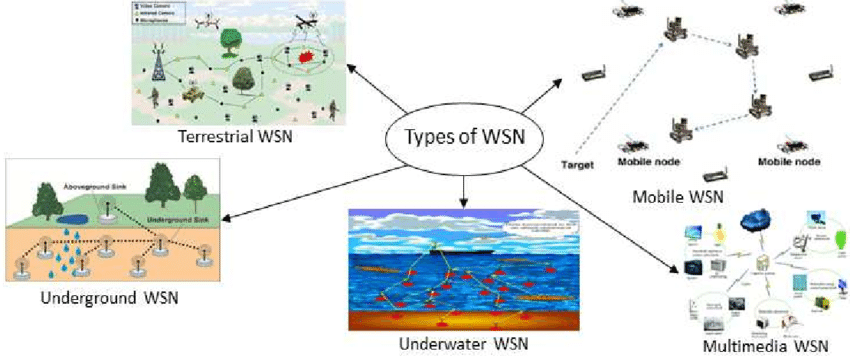
\includegraphics[width=0.8\textwidth]
		{images/wsn_types.png}}
	\caption{Các loại mạng cảm biến không dây}\label{fig:wsn-types}
\end{figure}

\subsection{Nút cảm biến}
Thành phần nhỏ nhất của một mạng cảm biến không dây là nút cảm biến. Cấu tạo của nút cảm biến bao gồm những bộ phận chính sau: bộ phận điều khiển, bộ phận chuyển tiếp, bộ nhớ, nguồn năng lượng, một hoặc nhiều bộ cảm ứng.
\begin{itemize}
	\item Các thành phần cảm ứng là các thiết bị phần cứng, liên tục đo đạc những thông số của môi trường xung quanh, như là áp suất hay nhiệt độ, sau đó chuyển các tín hiệu liên tục này thành các tín hiệu số để xử lý tiếp bằng các thành phần khác. Có thể phân loại thành phần cảm ứng thành 3 loại: bị động - đa hướng, bị động - đơn hướng hoặc chủ động. Các thiết bị bị động - đa hướng chỉ ghi nhận dữ liệu mà không tác động trực tiếp với môi trường. Dữ liệu ghi nhận bởi thiết bị này không chỉ ra hướng thu nhận được, khác với các thiết bị bị động - đơn hướng như camera. Các thiết bị chủ động thì tác động tới môi trường, ví dụ bằng tia rada, và chúng cần được liên tục cấp năng lượng.
	\item Bộ nhớ thì tùy thuộc vào yêu cầu mà được trang bị hay không. Vì mục tiêu tiết kiệm năng lượng mà bộ nhớ trên vi xử lý được ưu tiên hơn là bộ nhớ flash. Hai tác vụ chính của bộ nhớ bao gồm: lưu trữ dữ liệu và phục vụ cho tính toán.
	\item Bộ phận xử lý có thể coi như là bộ não của nút cảm biến, chịu trách nhiệm thực thi nhiệm vụ, xử lý dữ liệu và điều khiển các bộ phận khác. Lựa chọn phổ biến là sử dụng vi điều khiển bởi tính tiết kiệm, tiêu thụ ít năng lượng và dễ dàng lập trình.
	\item Bộ phận chuyển tiếp đóng vai trò cầu nối giữa các nút cảm biến, chịu trách nhiệm truyền và nhận các gói dữ liệu. Môi trường truyền tin sử dụng sóng radio, tia laze hoặc tia hồng ngoại. Tia laze thì sử dụng ít năng lượng, nhưng yêu cầu không gian truyền không được có vật cản. Tia hồng ngoại thì bị hạn chế bởi phạm vi giao tiếp. Bởi vậy phù hợp nhất với các ứng dụng của mạng cảm biến không dây là sử dụng sóng radio.
\end{itemize}
Vì thương được lắp đặt tại các vị trí khó tiếp cận, việc sạc hay thay pin dường như là không khả thi, bởi vậy mà nguồn năng lượng chính của các nút cảm biến thường sử dụng là pin. Các nút cảm biến tiêu tốn năng lượng cho các nhiệm vụ khác nhau, bao gồm: cảm ứng, xử lý dữ liệu và truyền dữ liệu. Trong đó việc truyền dữ liệu tiêu tốn năng lượng nhiều nhất.


Hình \ref{fig:wsn-nodes} mô tả cấu trúc của một nút cảm biến trong mạng cảm biến không dây.


\begin{figure}[htb]
	\center{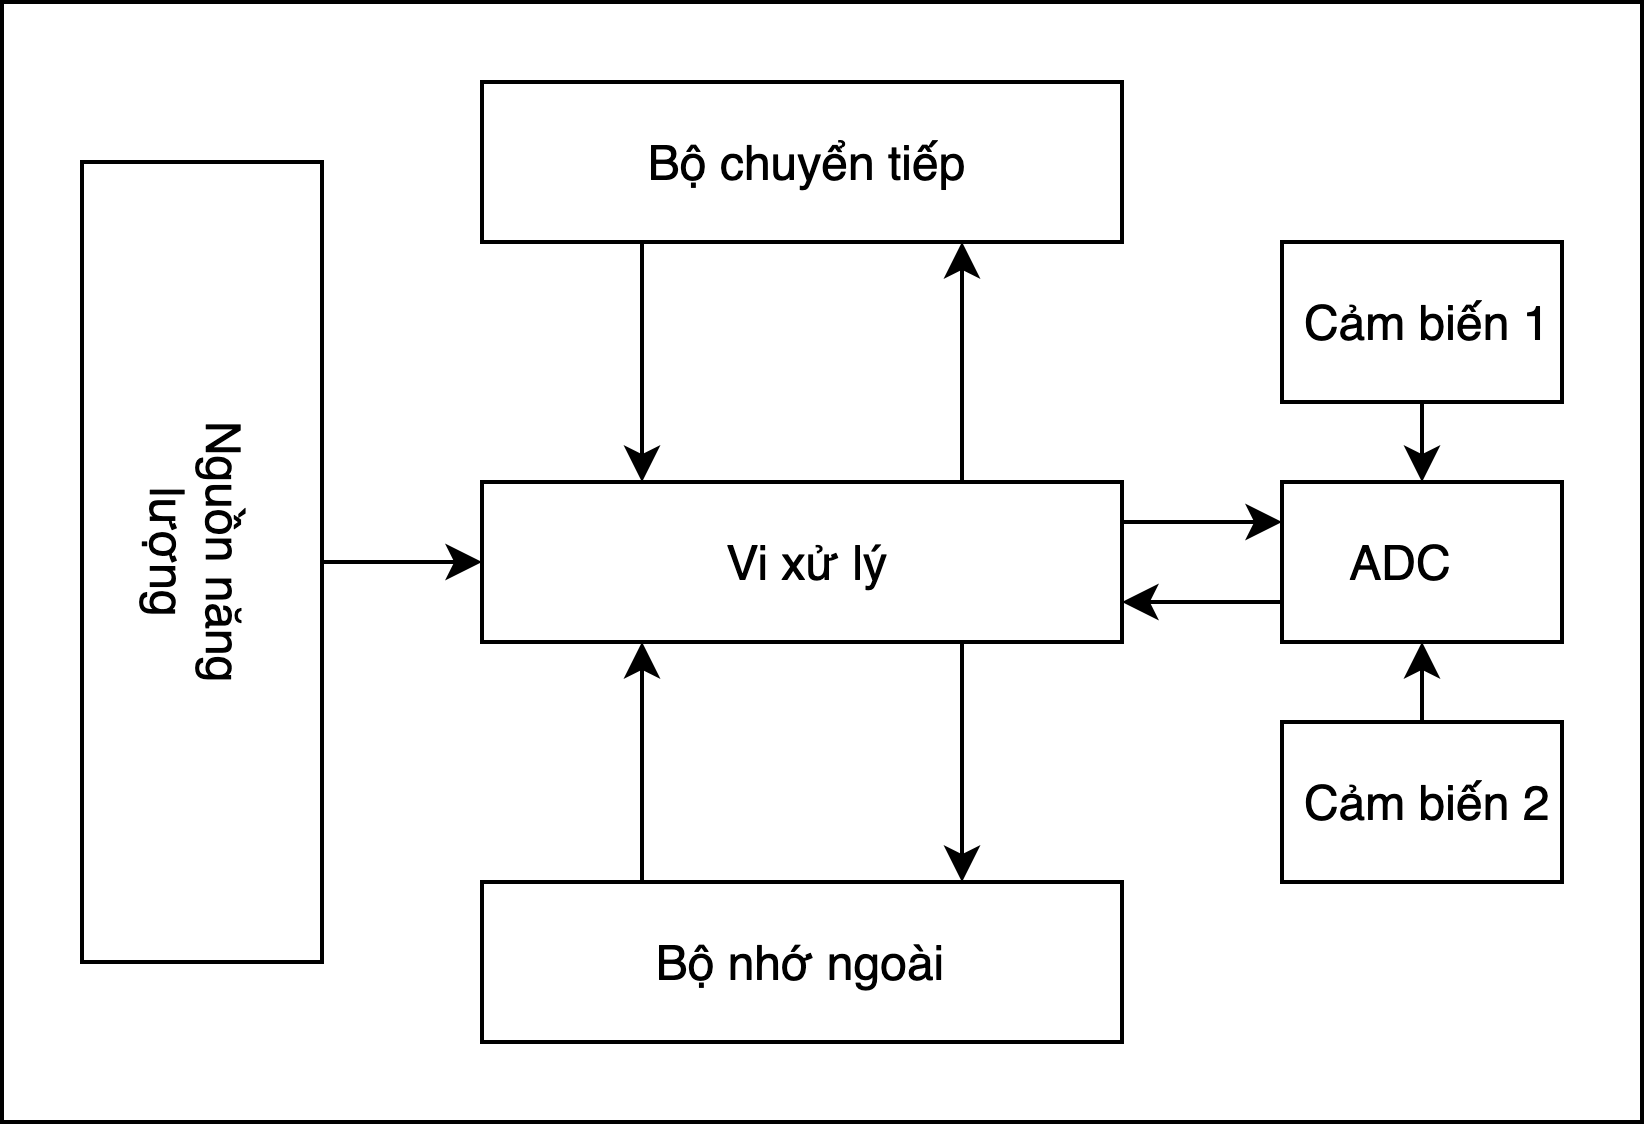
\includegraphics[width=10cm, height=8cm]
		{images/wsn_nodes.png}}
	\caption{Cấu trúc một nút cảm biến}\label{fig:wsn-nodes}
\end{figure}

\subsection{Các giao thức truyền tin của mạng cảm biến}
Mạng cảm biến không dây có thể được triển khai bằng nhiều giao thức \cite{akkaya2005survey}:


\begin{itemize}
	\item Dạng bus: Giao thức mạng đơn giản, được sử dụng khi có một số lượng ít nút cảm biến. Các nút thực hiện việc truyền tin qua hình thức quảng bá, tất cả các nút đều nhận được gói tin nhưng chỉ nút cảm biến đích là xử lý gói tin truyền tới. Tuy dễ dàng để cài đặt, giao thức dạng này cần phải có cơ chế xử lý xung đột hợp lý.
	\item Dạng cây: Giao thức dạng cây được xây dựng theo cơ chế kế thừa, các nút con (là các nút cảm biến) có trách nhiệm đo đạc thông tin môi trường và truyền ngược lại các nút cha (có thể là các nút cảm biến hoặc chỉ là các nút truyền tin) để xử lý. Vì việc truyền và nhận tin thường tiêu tốn nhiều năng lượng nhất (so với việc xử lý hay lưu trữ), bởi vậy mà cần tìm đường truyền ngắn nhất đi từ nút con tới nút gốc.
	\item Dạng hình sao: Giao thức này bao gồm một khu xử lý trung tâm nhận tất cả thông tin từ các nút xung quanh để xử lý. Tất cả việc giao tiếp đều phải thực hiện thông qua khu trung tâm này (giống với mô hình client - server). 
	\item Dạng hình vòng: Các nút trong giao thức này được kết nối với chính xác 2 nút khác, việc truyền tin do đó được thực hiện tuần tự theo chiều kim đồng hồ hoặc ngược kim đồng hồ. Nếu có một nút bị chết thì toàn bộ mạng phải có cơ chế hồi phục lại.
	\item Dạng hỗn tạp (Mesh Network): Giao thức mạng cho phép một nút có thể giao tiếp với các nút kề với nó, đồng thời có thể truyền tin theo nhiều hướng tới nút đích (khác với mạng hình vòng chỉ cho truyền theo 2 hướng).
	\item Dạng kết nối đầy đủ (Fully connected network): Giao thức mạng mà một nút kết nối với tất cả các nút khác trong mạng. Số lượng nút và số lượng kết nối giữa tất cả các nút tăng theo hàm lũy thừa khiến cho việc tính toán đường đi tối ưu cho gói tin rất khó khăn.
\end{itemize}

Hình \ref{fig:wsn-topology} tổng hợp của các giao thức thường được triển khai trong thực tế.


\begin{figure}[htb]
	\center{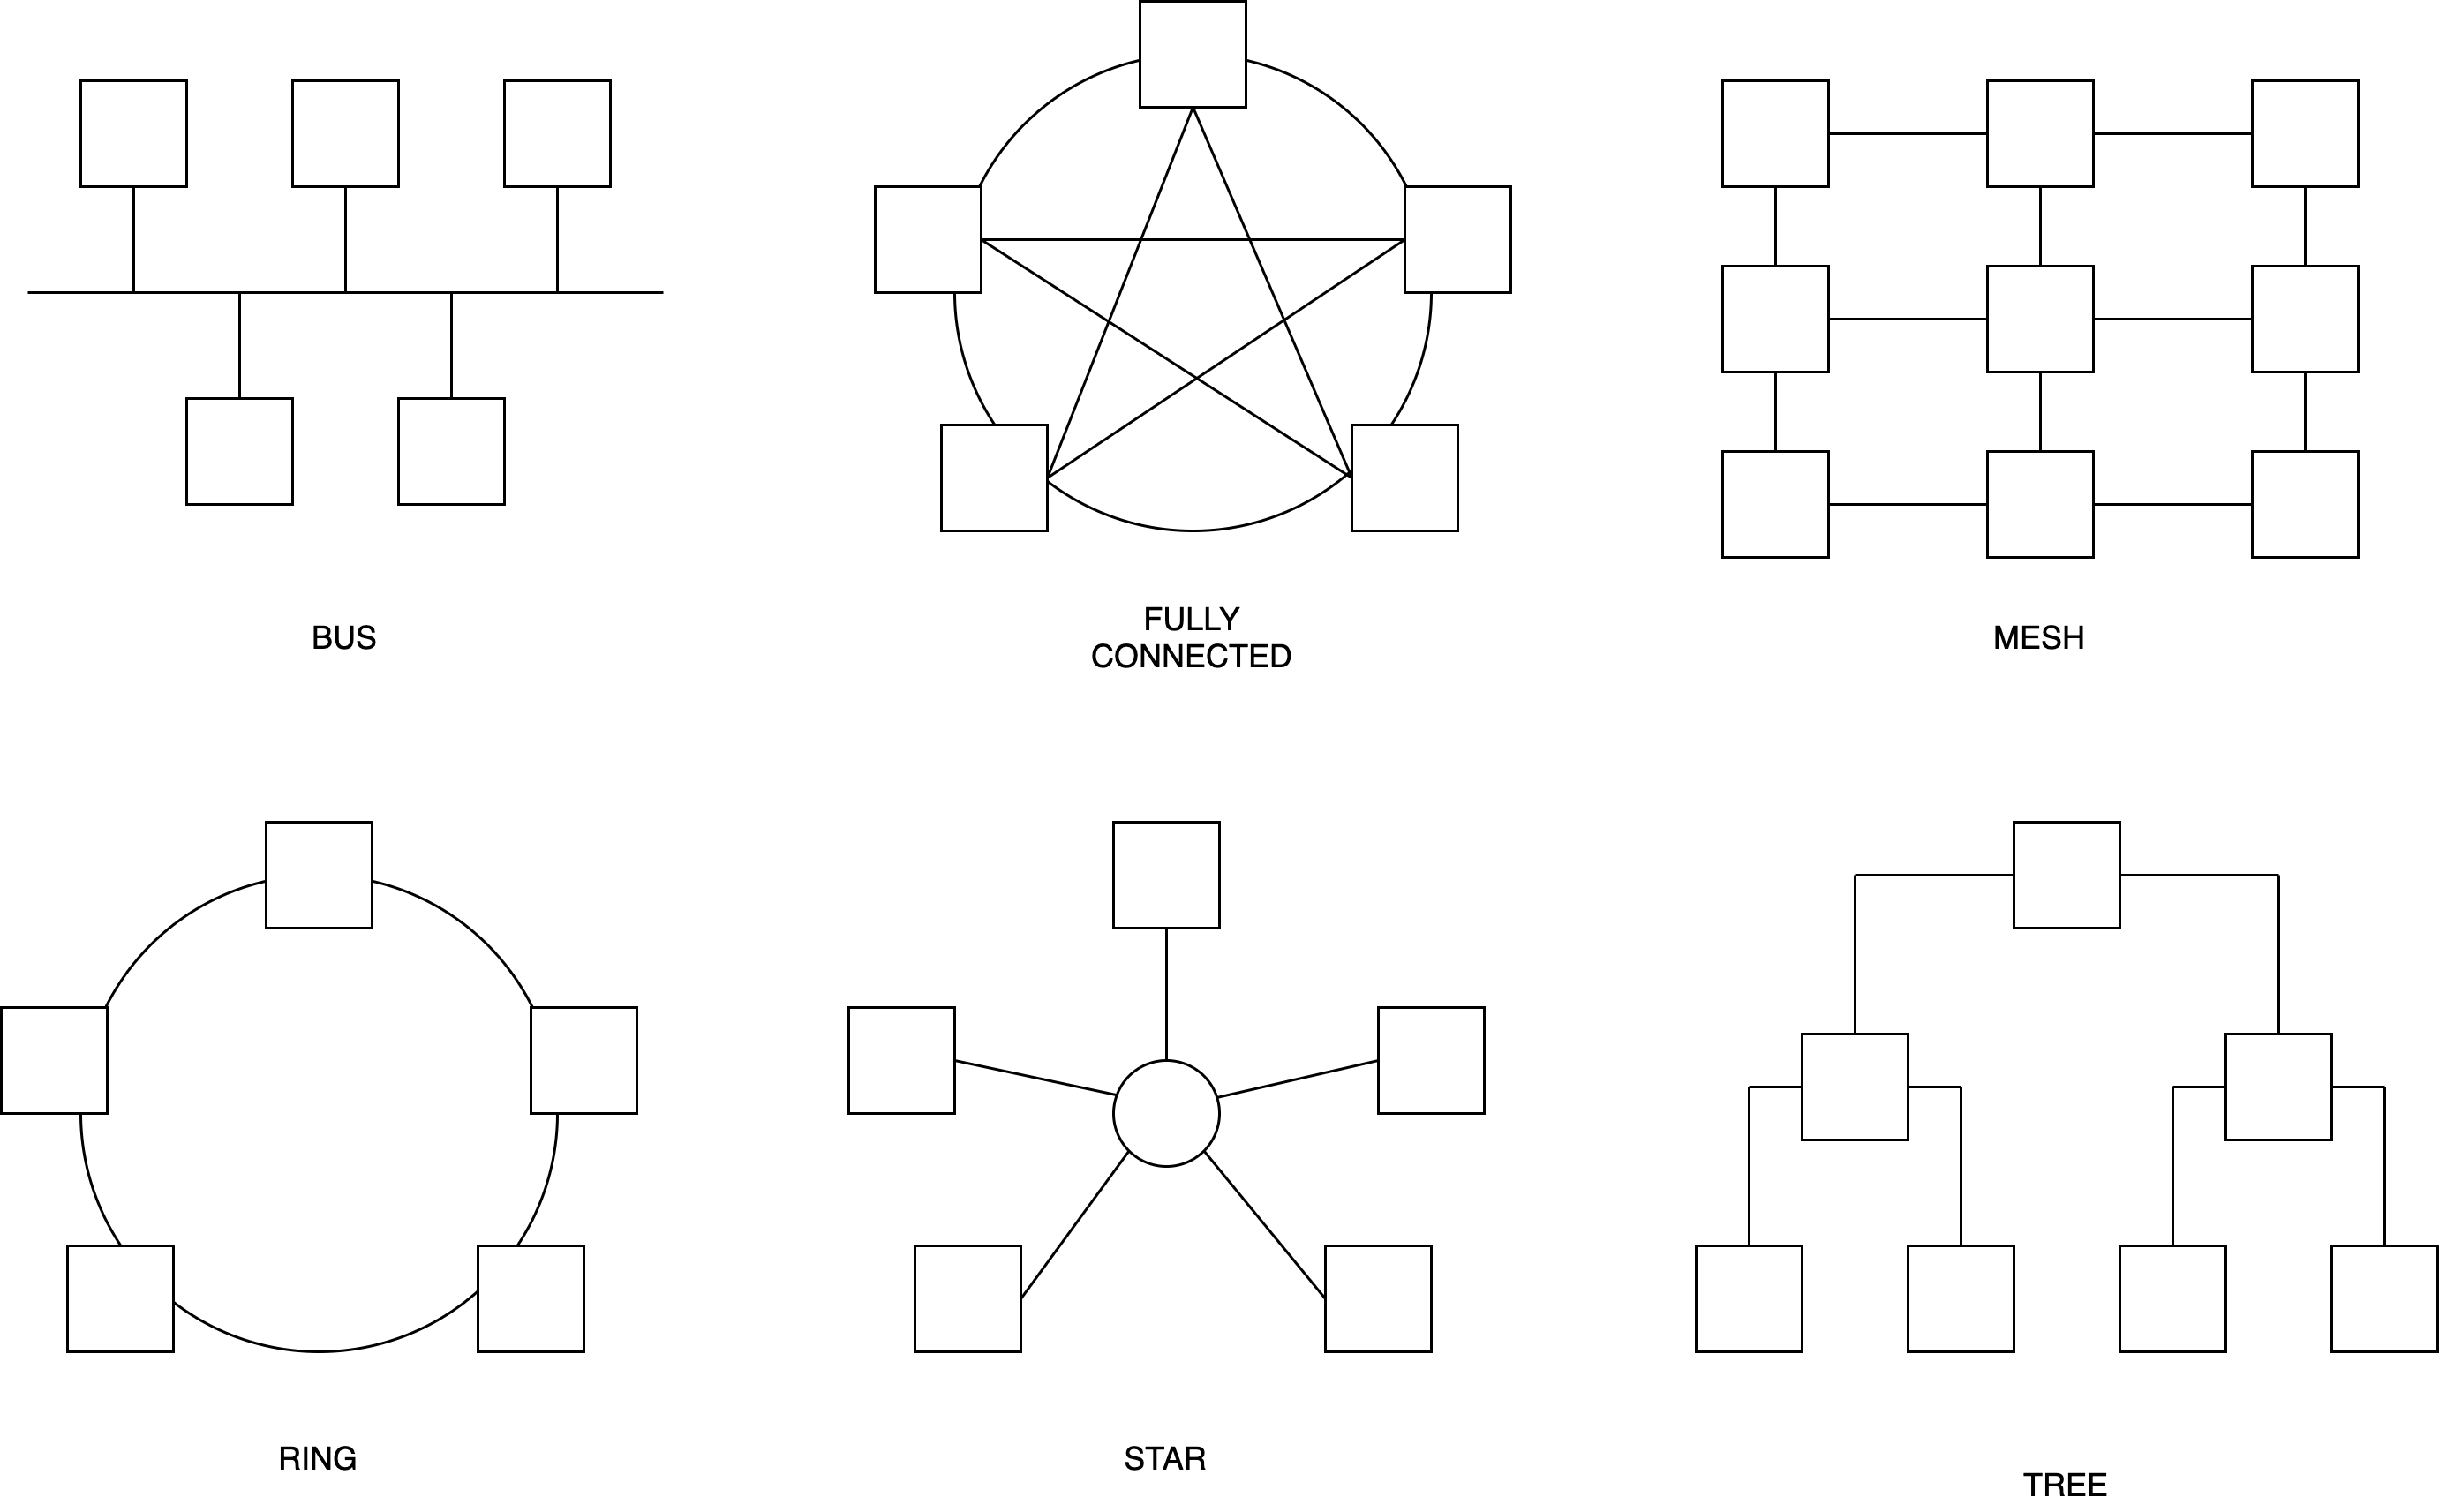
\includegraphics[width=0.8\textwidth, height=8cm]
		{images/wsn_topology.png}}
	\caption{Các giao thức mạng trong thực tế}\label{fig:wsn-topology}
\end{figure}

\subsection{Ứng dụng của mạng cảm biến không dây}
Mạng cảm biến không dây từ những ngày đầu chỉ được ứng dụng trong quân sự và khoa học nay đã phát triển rộng rãi và cho thấy tác dụng lớn khi áp dụng vào trong những mặt khác của đời sống như: nông nghiệp, y tế, môi trường, xây dựng. Việc nhận thấy tiềm năng của mạng cảm biến không dây trong nhiều lĩnh vực của xã hội thúc đẩy khoa học và doanh nghiệp đẩy mạnh nghiên cứu, hợp tác để cho ra đời những nút cảm biến hiệu quả hơn, tiết kiệm hơn và các cơ chế triển khai mạng cảm biến tối ưu hơn. Dưới đây là bản nghiên cứu tác động của mạng cảm biến không dây trong các lĩnh vực khác nhau \cite{ramson2017applications}:
\begin{itemize}
	\item Nông nghiệp: Các mạng cảm biến kết hợp của nhiều loại như dưới đất, trong lòng đất hay trong nước cung cấp thông tin cần thiết cho canh tác như nhiệt độ, độ ẩm, chất lượng đất, số lượng khí CO2 trong lòng đất, chất lượng nước. Dữ liệu được thu thập qua camera hoặc cảm biến, sau đó được xử lý và đưa tới chuyên gia để đưa ra quyết định sau cùng. Nhờ thông tin được truyền tải theo thời gian thực mà chuyên gia có thể phân tích tình trạng cây trồng, đất đai, nguồn nước để có cơ chế điều chỉnh thích hợp. Ngoài việc ghi nhận thông tin, các mạng cảm biến còn đóng vai trò tự động hóa quy trình canh tác, điều khiển để giảm thiểu công sức lao động, tăng năng suất và độ chính xác, giống như hệ thống thời gian thực được điều khiển bằng cảm biến tại các khu trồng trọt trong nhà kính.
	\item Môi trường: Nhờ việc ghi nhận dữ liệu và truyền tải qua Internet mà có thể dự đoán trước các thiên tai tự nhiên như động đất, sóng thần, lũ lụt hay tai nạn lao động như rò rỉ khí ga, rò điện, qua đó giảm thiểu thiệt hại về người và của. Các ứng dụng thực tiễn trong môi trường có thể kể đến giám sát mức độ ô nhiễm môi trường, giám sát chất lượng nước và khí thải trong nhà máy, dự đoán nguy hiểm trong hầm mỏ như khí độc, nguồn lửa ngầm hoặc sập hầm. 
	\item Giao thông: Giám sát giao thông là một ví dụ thực tiễn của mạng cảm biến truyền thông, kết hợp nhiều camera giám sát để thu được hình ảnh thời gian thực, hỗ trợ việc điều tiết, phân luồng, truy cứu trách nhiệm khi có tai nạn, xử lý vi phạm giao thông. Hệ thống giám sát giao thông đã được triển khai ở rất nhiều thành phố lớn trên thế giới giúp giảm thiểu lực lượng công quyền cần có mặt trực tiếp trên đường. 
	\item Y tế: Các mạng cảm biến không dây được triển khai để giám sát sức khỏe của bệnh nhân, cụ thể là đo đạc thông số cơ thể như áp suất, chất béo, đặc biệt là ở người già, để có thể liên tục theo dõi và chăm sóc tình trạng. Bệnh nhân có thể đeo các thiết bị đo đạc và hệ thống sẽ tự động gửi thông tin về trung tâm liên tục để bác sĩ có thể chẩn đoán và đưa ra phác đồ điều trị một cách chính xác nhất.
	\item Quân sự: Vai trò của mạng cảm biến không dây vẫn chưa hề mờ nhạt trong lĩnh vực quân sự, thậm chí là các mạng cảm biến hiện thời còn mang lại nhiều giá trị hơn. Giám sát kẻ địch, phát hiện xâm nhập, tính toán toán lộ trình là các mục tiêu chính khi triển khai mạng cảm biến không dây trên chiến trường.
\end{itemize}

\subsection{Khó khăn}
Như đã đề cập ở đầu chương, việc được ứng dụng rộng rãi ở nhiều lĩnh vực thúc đẩy những tiến bộ khoa học nhưng đồng thời cũng mang tới những thách thức khi triển khai một mạng cảm biến không dây trong thực tế \cite{eisa2013challenges}. 


Một trong những thách thức lớn nhất và được ưu tiên hàng đầu khi thiết kế mạng cảm biến không dây là duy trì thời gian sống. Bởi đặc tính khó tiếp cận của môi trường đặt các nút cảm biến (trong lòng đất, trên chiến trường) vậy nên việc sạc pin cho các mạng cảm biến hay đổi pin mới dường như là không thể. Hơn thế nữa với các giao thức mạng hình cây hoặc hình vòng, một nút chết trong mạng có thể dẫn tới việc tái định tuyến cho toàn bộ các nút khác. Từ hai nguyên do trên mà trước khi bắt đầu triển khai các nút cảm biến (có thể là chọn vị trí đặt hoặc xác định thuật toán định tuyến, giao thức truyền, giao thức xử lý xung đột), các kĩ sư đều phải lưu ý tới việc giảm thiểu năng lượng tiêu thụ. Nhưng bởi số lượng kênh hạn chế, lại cần phải được chia sẻ giữa rất nhiều nút mạng, điều này có thể dẫn tới độ trễ lớn nếu quá ưu tiên vào việc bảo vệ năng lượng, khiến cho thông tin trở nên vô giá trị. Cân bằng giữa việc duy trì thời gian sống và đảm bảo hiệu quả trong giao tiếp là một bài toán khó, với những yêu cầu thay đổi tùy vào tình hình thực tế.


Ở những môi trường có khả năng xảy ra hư hại cho các nút cảm biến (chiến trường), một cơ chế chịu lỗi hay tái định tuyến là cần thiết để đảm bảo giao tiếp trong toàn mạng khi có vấn đề xảy ra. Ví dụ, một nút cần cập nhật lại bảng địa chỉ các mạng khác khi nhận thấy việc truyền tin như trước không hiệu quả. Cơ chế chịu lỗi cùng với cơ chế tự vận hành, khi các nút trong mạng đã được thiết lập thì có thể tự động thực hiện tác vụ mà không cần tới sự có mặt của con người, hỗ trợ cho tính tự động hóa của mạng cảm biến không dây, giảm thiểu chi phí lao động.


Đôi khi, các mạng cảm biến không dây cần được thiết kế để đảm bảo độ phủ trong truyền tin hay thông tin cần được truyền trong thời gian thực. Độ bao quát của mạng cảm biến phục vụ cho mục đích giám sát tổng quát như các lưới bảo vệ tại các cứ điểm quan trọng để phát hiện quân địch hay các khu vực rộng lớn như đất ruộng canh tác để thu thập đầy đủ dữ liệu. Trong khi đó đảm bảo chất lượng dịch vụ là một trong những yêu cầu của mạng truyền thông bởi con người rất nhạy cảm với độ trễ của âm thanh hay hình ảnh. Việc đảm bảo chất lượng đường truyền, chất lượng gói tin, trong khi vẫn duy trì thời gian sống của mạng là một thách thức không nhỏ.

\section{Lý thuyết đồ thị}
\subsection{Định nghĩa và biểu diễn đồ thị}
Đồ thị, trong phạm vi toán học, là một tập hợp những đối tượng được mã hóa thành các đỉnh và mối liên hệ giữa các đối tượng được mã hóa dưới dạng cạnh. 


Hình \ref{fig:undirected_graph} là một đồ thị đơn vô hướng.


\begin{figure}[htb]
	\center{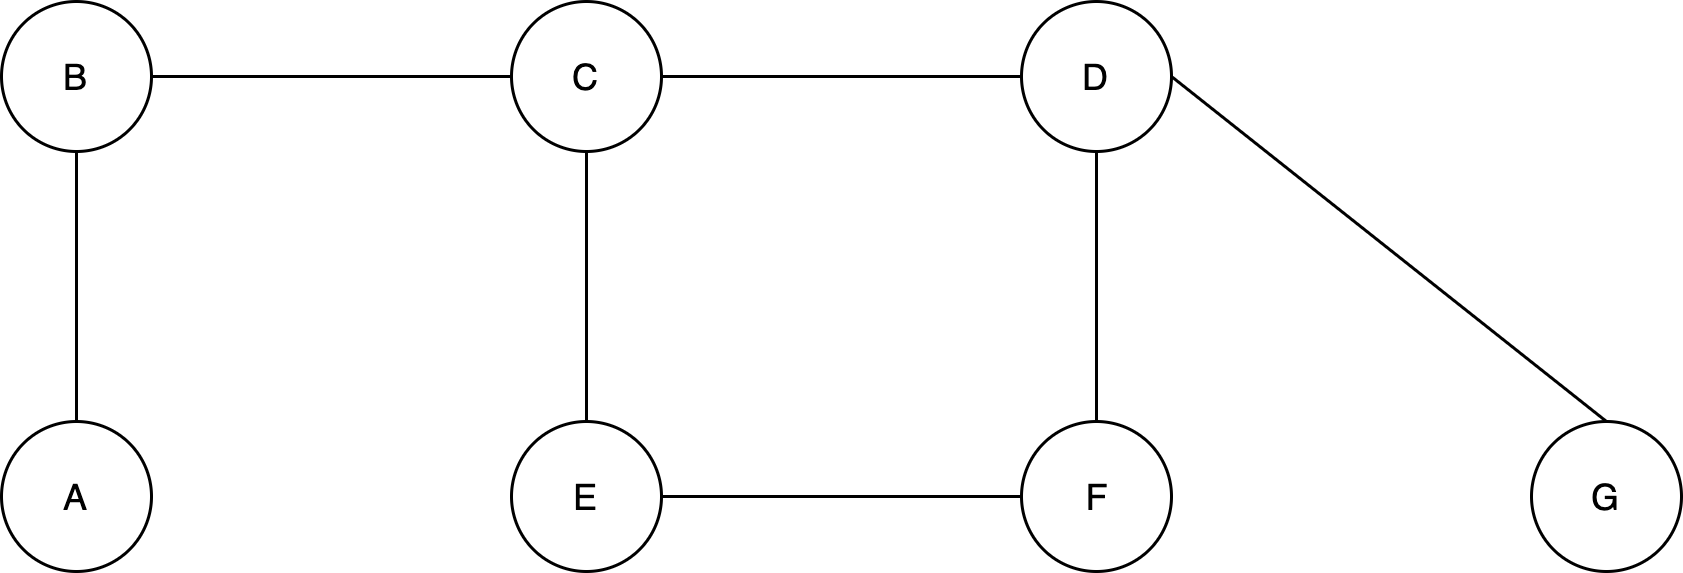
\includegraphics[width=0.8\textwidth, height=5cm]
		{images/undirected_graph.png}}
	\caption{Đồ thị đơn vô hướng}\label{fig:undirected_graph}
\end{figure}

Đồ thị có thể được sử dụng để mô hình hóa rất nhiều bài toán trong thực tế \cite{sedgewick2011algorithms}:
\begin{itemize}
	\item Bản đồ: Một bản đồ giữa các thành phố có thể là một đồ thị, trong đó các thành phố là các đỉnh, đường đi từ thành phố A tới thành phố B gần đó là một cạnh của đồ thị. Việc mô hình hóa như này có thể giúp giải các bài toán như xác định đường đi ngắn nhất từ một thành phố tới thành phố khác bằng các giải thuật trên đồ thị.
	\item Internet: Các trang web trên mạng là các đỉnh của đồ thị và các hyperlink là các cạnh của đồ thị. Các thuật toán duyệt đồ thị đóng vai trò quan trọng trong các bộ công cụ tìm kiếm.
	\item Lập lịch: Cơ chế lập lịch xuất hiện từ những nơi bé nhất như hệ điều hành cho tới nhà máy, sân bay. Việc lập một kế hoạch hợp lý, đáp ứng yêu cầu, đảm bảo một số ràng buộc như tài nguyên hay độ ưu tiên có thể được xử lý trước hết bằng cách mô hình hóa bằng đồ thị có hướng, sau đó áp dụng các thuật toán sắp xếp hoặc tìm kiếm đường đi trên đồ thị.
\end{itemize}
Tùy thuộc vào yêu cầu bài toán mà có thể lựa chọn mô hình đồ thị phù hợp, vô hướng hoặc có hướng, cạnh có trọng số hoặc không. Với đồ thị vô hướng, chiều cạnh nối 2 đỉnh là không quan trọng, có thể duyệt từ A tới B hoặc từ B tới A đều được, nếu tồn tại cạnh giữa 2 đỉnh A và B. Trong khi đó với đồ thị có hướng, giả sử hướng từ A tới B thì chỉ có thể duyệt từ A tới B. Chúng ta thường mô hình hướng của cạnh trong đồ thị bằng cách thêm dẫu mũi tên vào đích của cạnh, biểu thị chiều từ nguồn tới đích. Với trường hợp trọng số của cạnh, với các bài toán mà việc di chuyển từ đỉnh này tới đỉnh khác tiêu tốn tài nguyên (xăng dầu khi di chuyển trên đường, thời gian hoàn thành tác vụ,v.v...), các cạnh nối giữa 2 đỉnh sẽ được đánh trọng số thể hiện số tài nguyên sẽ tiêu tốn khi di chuyển trên cạnh này.


Cùng tùy thuộc vào yêu cầu của bài toán mà cách lưu trữ đồ thị trong bộ nhớ cũng khác nhau, nhưng có thể lựa chọn cách lai ghép để thu được hiệu quả từ cả 2. Cách lưu trữ sử dụng ma trận nhị phân, mà phần tử $a_{ij}$ là 0 hoặc 1 chỉ việc có tồn tại cạnh giữa 2 đỉnh i và j của đồ thị, sẽ tăng tốc việc truy cập nhưng lại tiêu tốn bộ nhớ. Trong khi đó nếu sử dụng các danh sách liên kết mà phần từ đầu là các đỉnh và các phẩn từ trong danh sách là các đỉnh liên kết với nó sẽ giúp giảm thiểu bộ nhớ sử dụng, nhưng tất nhiên việc truy xuất sẽ tiêu tốn thời gian hơn.

\subsection{Thuật toán duyệt đồ thị}
Duyệt đồ thị được hiểu là ghé thăm tất cả các đỉnh ở đồ thị (hoặc cho tới khi tìm được đỉnh cần thiết), mỗi đỉnh đúng một lần. Thuật toán duyệt đồ thị có thể được sử dụng như một cơ chế tiền xử lý cho các bài toán phức tạp khác như xác định chu trình hay tìm đường đi ngắn nhất.


Bên dưới là thuật toán \Gls{BFS}., là thuật toán sẽ thăm tất cả các đỉnh ở mức hiện tại (các nút kề với đỉnh đã xét gần nhất) trước khi thăm các đỉnh ở mức khác.

\begin{algorithm}
	\caption{Breadth-first search}\label{euclid}
	\begin{algorithmic}[1]
		\Procedure{BFS}{$Graph, Key$}
		\State Tạo hàng đợi rỗng
		\State Thêm nút gốc vào hàng đợi
		\State Tạo tập hợp các nút đã thăm
		
		\While {Hàng đợi vẫn chưa rỗng}
		\State nút $\leftarrow$ đầu hàng đợi
		\State Kiểm tra khóa của nút
		\State Thêm nút vào tập hợp đã thăm
		\State Thêm vào hàng đợi tất cả các đỉnh lân cận chưa được thăm của nút được xét gần nhất
		\EndWhile
		\EndProcedure
	\end{algorithmic}
\end{algorithm}


\Gls{DFS} ngược lại so với \gls{BFS} khi chúng ta ưu tiên thăm các đỉnh theo chiều sâu trước khi mở rộng ra các đỉnh lân cận.


\begin{algorithm}
	\caption{Depth-first search}\label{euclid}
	\begin{algorithmic}[1]
		\Procedure{DFS}{$Graph, Key$}
		\State Tạo stack rỗng 
		\State Thêm vào stack nút gốc
		\State Tạo tập hợp các nút đã thăm 
		
		\While {Stack vẫn chưa rỗng}
		\State nút $\leftarrow$ pop stack
		\State Kiểm tra khóa của nút
		\State Thêm vào stack tất cả các đỉnh lân cận chưa được thăm của đỉnh được xét gần nhất
		\EndWhile
		\EndProcedure
	\end{algorithmic}
\end{algorithm}

\subsection{Thuật toán xây dựng cây khung nhỏ nhất}
Cây khung nhỏ nhất là một đồ thị liên thông không có chu trình nối tất cả các đỉnh trong đồ thị. Hai thuật toán xây dựng cây khung nhỏ nhất được trình bày bên dưới là Kruskal và Prim.

\begin{algorithm}
	\caption{Thuật toán Kruskal}\label{euclid}
	\begin{algorithmic}[1]
		\Procedure{Kruskal}{$Graph$}
		\State Tạo một rừng với mỗi đỉnh là một cây độc lập.
		\While {Cây khung nhỏ nhất chưa hình thành}
		\State Loại bỏ một cạnh từ tập E với trọng số nhỏ nhất.
		\If {Hai đỉnh trên cạnh thuộc về hai cây khác nhau}
		\State Kết hợp thành một cây.	
		\EndIf	
		\EndWhile 
		\EndProcedure
	\end{algorithmic}
\end{algorithm}

\begin{algorithm}
	\renewcommand{\thealgorithm}{}
	\caption{Thuật toán Prim}\label{euclid}
	\begin{algorithmic}[1]
		\Procedure{Prim}{$Graph$}
		\State Gán trọng số cho mỗi đỉnh.
		\While {Cây khung nhỏ nhất chưa hình thành}
		\State Lựa chọn đỉnh v có trọng số nhỏ nhất thêm vào cây.
		\State Cập nhật trọng số cho các đỉnh liền kề với v nếu chi phí di chuyển từ v nhỏ hơn trọng số hiện tại.
		\EndWhile 
		\EndProcedure
	\end{algorithmic}
\end{algorithm}

\subsection{Lý thuyết về cây trong đồ thị}
Cây, trong mối liên quan với đồ thị, có thể được xem như một đồ thị liên thông, không có chu trình, trong đó ta chọn ra một đỉnh gọi là gốc. Hình ảnh trực quan là dễ dàng nhất để giúp định nghĩa những thành phần trong cây.

\begin{figure}[htb]
	\center{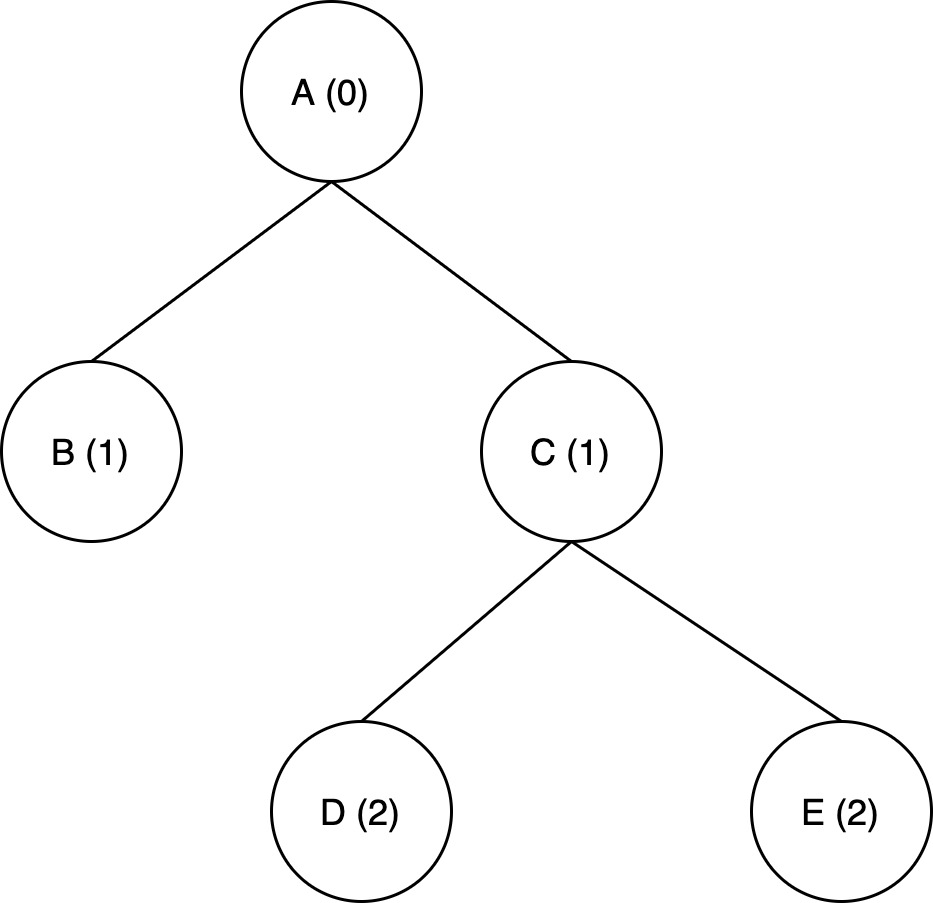
\includegraphics[width=5cm, height=5cm]
		{images/tree.jpg}}
	\caption{Cây trong lý thuyết đồ thị.}\label{fig:tree}
\end{figure}


Các thành phần của một cây khi quan sát từ hình \ref{fig:tree} bên trên sẽ bao gồm: nút A là nút gốc, nút B, C là các nút con của và tương ứng nút A là cha của chúng (nút C là cha của 2 nút D,E và D,E là con của C). (Vì chúng ta chỉ đề cập tới cây tổng quát nên sẽ không có khái niệm con trái hay con phải). Các nút D,E được gọi là các nút lá nếu không có bất kỳ con nào. Một cây có nhiều mức, các cây cùng một cha sẽ cùng một mức (hoặc có cha cùng mức thì cũng có cùng mức) và sẽ có mức lớn hơn mức cha là 1. Bắt đầu từ nút gốc có mức 0, các nút B,C sẽ có mức 1, D,E có mức 2. Chiều cao của cây là đường dài nhất đi từ gốc tới nút lá bất kỳ, hay được tính đơn giản bằng mức sâu nhất.

\subsubsection{Cây Steiner}
Trong phạm vi tổng quát, cây Steiner là một tập các bài toán trong lĩnh vực tổi ưu hóa tổ hợp. Nhưng để tập trung vào vấn đề tiếp theo sẽ giải quyết ở chương 2, chúng ta chỉ quan tâm tới cây Steiner trong đồ thị, có thể được diễn giải một cách đơn giản như sau: một cây Steiner là một cây có trọng số nhỏ nhất chứa tất cả những đỉnh cần thiết (là một tập con của tất cả các đỉnh trong đồ thị), cây có thể bao gồm các đỉnh khác hoặc không. Khái niệm trọng số nhỏ nhất ở đây có thể hiểu là tối thiểu hóa hàm mục tiêu (các mục tiêu có thể là thời gian sống trong mạng, độ bao phủ của các nút cảm biến, độ trễ của đường truyền) đối với các bài toán trong mạng cảm biến không dây. Khi số lượng nút Steiner (các nút bắt buộc xuất hiện trong cây) bằng với số nút trong đồ thị, ta có thể quy về bài toán cây khung nhỏ nhất. Còn khi chỉ có 2 nút Steiner thì ta có thể quy về bài toán đường đi ngắn nhất. Mặc dù vậy, tuy 2 bài toán trên có thể giải trong thời gian đa thức, cây Steiner lại thuộc lớp NP-complete \cite{karp1972reducibility}.

\section{Tổng kết}
Chương 1 bao gồm những kiến thức tổng quan về lĩnh vực mà đồ án nghiên cứu (mạng cảm biến không dây), và một số phạm trù khoa học máy tính liên quan tới bài toán đặt ra (đồ thị và cây Steiner). Cụ thể, phần 1.1 cho biết những giao thức mạng thường được sử dụng, ứng dụng và khó khăn khi triển khai một mạng cảm biến không dây trong thực tế. Kiến thức trong phần này có thể giúp những người mới tiếp cận dễ dàng hơn với một trong những lĩnh vực đang thu hút nhiều sự quan tâm của giới nghiên cứu cũng như có cái nhìn bao quát về sự hiện diện của mạng cảm biến không dây trong đời sống. Phần 1.2 đóng vai trò như sự bổ sung kiến thức cho phần diễn giải chi tiết ở chương sau, đặc biệt là phần giải mã của các thuật toán sẽ được áp dụng đã được trình bày chi tiết, cụ thể là thuật toán \gls{BFS} để duyệt cây và Kruskal để xây dựng cây con nhỏ nhất.

\chapter{Bài toán tối ưu cây Steiner tổng hợp dữ liệu đa mục tiêu}
Sự tiến bộ của công nghệ giúp sản xuất các thiết bị cảm biến ngày một hiện đại, chiếm ít không gian, hiệu năng cao, giá thành rẻ, hỗ trợ triển khai số lượng lớn trên cùng một không gian. Đi liền với đó là khó khăn trong việc tận dụng hiệu quả các nút cảm biến khi năng lượng, khả năng tính toán, bộ nhớ vẫn còn hạn chế. Tổng hợp dữ liệu được nghiên cứu nhằm giải quyết khó khăn này. Nhiệm vụ này được định nghĩa như một quy trình toàn cục bao gồm việc tập trung và điều hướng thông tin thông qua các lớp mạng, xử lý dữ liệu tại các nút trung gian nhằm giảm thiểu việc tiêu thụ năng lượng, qua đó duy trì thời gian sống toàn mạng \cite{fasolo2007network}.


Các tác vụ trong tổng hợp dữ liệu có thể kể đến: giao tiếp thông tin giữa các nút cảm biến, tính toán, tổng hợp tại một nút và lưu trữ dữ liệu. Trong thực tế, việc giao tiếp thông tin giữa các nút cảm biến thường tiêu hao nhiều năng lượng nhất. Tác vụ này bao gồm rất nhiều phương pháp điều hướng gói tin trong mạng, hỗ trợ cho việc tổng hợp dữ liệu từ nhiều nguồn và truyền tải tới một (hoặc nhiều) đích đến. Một số giao thức hỗ trợ giao tiếp thông tin trong mạng có thể kể đến: giao thức dạng cây, giao thức dạng cụm, giao thức đa đường và giao thức lai.


Giao thức dạng cây là phương thức cổ điển để tổng hợp dữ liệu trong mạng cảm biến không dây, trong đó các nút cảm biến được tổ chức theo cấu trúc phân cấp và kế thừa. Trước hết, một cây với trạm tiếp nhận thông tin là nút gốc được xây dựng. Sau đó việc truyền và nhận thông tin được thực hiện tuần tự theo từng cấp, từ lá tới gốc. Giao thức này phù hợp để áp dụng trong các bài toán tối ưu hóa các hàm tổng hợp dữ liệu và và quản lý năng lượng \cite{fasolo2007network}. 


Trong thực tế, không phải lúc nào tất cả các nút được triển khai cũng truyền tải dữ liệu, chỉ một số các nút được chỉ định là các nút cảm biến có nhiệm vụ thu thập dữ liệu xung quanh và truyền lên các cấp cao hơn. Bài toán lúc này trở thành bài toán cây Steiner: tìm cây khung nhỏ nhất chứa tập con từ tập các đỉnh cho trước.


\section{Mô hình năng lượng}
Mô hình mất mát năng lượng ở \cite{heinzelman2002application} được áo dụng. Công thức tính toán năng lượng nhận và truyền dữ liệu có dạng như sau:
\begin{equation}
E_{RX} = k \times E_{elec}.
\end{equation}

\begin{equation}
E_{TX} = 
\begin{cases}
k \times E_{elec} + k \times \epsilon_{fs} \times d^2,  & d < d_0\\
k \times E_{elec} + k \times \epsilon_{mp} \times d^4, & d \geq d_0.\\
\end{cases}
\end{equation}

d là khoảng cách thực tế giữa các nút. $epsilon_{fs}$ và $epsilon_{mp}$ là các hằng số để tính toán năng lượng tiêu thụ khi truyền gói tin trong khoảng cách ngắn và khoảng cách dài.

Năng lượng tổng hợp dữ liệu $E_{DA}$ tại các nút là một hằng số.


\section{Phát biểu bài toán} \label{problem}
\begin{itemize}
	\item 
	Đầu vào: Mạng cảm biến không dây được triển khai trên địa hình ba chiều, mô phỏng theo chuẩn Digital Elevation Model \cite{mukherjee2013evaluation}. Trong đó, trạm trung tâm được đặt ở chính giữa của địa hình, các nút cảm biến được phân bố theo các phân phối và có vị trí cố định. 
	\begin{itemize}
		\item
		Tập các nút bao gồm $\{s_{1},s_{2},...,s_{n},r_{1},r_{2},...,r_{m},BS\}$. $s_{i}$ và $r_{j}$ là nút cảm biến thứ i và nút trung gian thứ j, BS là trạm trung tâm. Tọa độ của các nút được kí hiệu là $(x,y,z)$ tương ứng với giá trị theo độ rộng, độ dài và độ cao trong không gian.
		\item
		Bán kính giao tiếp các nút là $r_{c}$.
	\end{itemize}
	Một nút u có thể giao tiếp với một nút v nếu nút u nằm trong bán kính truyền thông của nút v và ngược lại. Bán kính truyền thông giữa hai nút là tổng của bán kính giao tiếp của từng nút, trong bài toán hiện tại là $2*r_{c}$. Do đó, mạng cảm biến không dây có thể được mô hình dưới dạng đồ thị $G = (V,E)$ trong đó V là tập các nút (bao gồm cả nút cảm biến và nút trung gian) và E là tập các cặp nút (u,v) có khả năng giao tiếp với nhau. Tập các nút trung gian trong cây Steiner được kí hiệu là RN (|RN| $\leq$ m).
	
	\item
	Đầu ra:  Cây khung Steiner T = $(V_{n+|RN|},E_{n+|RN|})$ với n là số lượng các nút cảm biến.
	
	\item
	Các mục tiêu:
	\begin{itemize}
		\item{Tổng năng lượng tiêu thụ} \\
		Vấn đề lớn nhất đối với các mạng cảm biến không dây là việc suy hao năng lượng của các nút cảm biến. Bởi các nút cảm biến dự trữ rất ít năng lượng, việc áp dụng các thuật toán nhằm tối thiểu hóa năng lượng tiêu thụ trong quá trình vận hành là vô cùng cần thiết. Năng lượng tiêu thụ của cây tổng hợp dữ liệu có thể được tính bằng tổng năng lượng trên tất cả các nút.
		
		\begin{equation}
		f_1(x) = \sum_{i=1}^{n + |RN|} (E^i_{TX} + \sum_{j=1}^{C_{num_i}} (E_{RX}^j + E_{DA}^j))
		\end{equation}
		
		$C_{num_i}$ là tất các nút con của nút thứ i trong cây tổng hợp dữ liệu. Năng lượng tiêu thụ trên mỗi nút sẽ bằng tổng của năng lượng truyền gói tin cho nút cha của nó và năng lượng tổng hợp (bao gồm năng lượng nhận gói tin và năng lượng tổng hợp dữ liệu) từ tất cả các nút con.
		
		\item{Thời gian sống của mạng} \\
		Một trong những mục tiêu khi triển khai mạng cảm biến không dây là duy trì thời gian sống toàn mạng. Bởi đặc điểm gồ ghề, khó tiếp cận của một số địa hình khi triển khai gây khó khăn cho việc thay thế, khắc phục sự cố như hết pin, tai nạn hay phá hoại từ bên ngoài mà việc duy trì tính ổn định là vô cùng cần thiết. Tùy thuộc vào yêu cầu thực tế mà định nghĩa thời gian sống của mạng cảm biến thay đổi: thời gian mà mạng cảm biến vẫn còn duy trì việc giao tiếp như thông thường, thời gian mà mạng cảm biến vẫn còn bao quát một không gian, thời gian từ khi bắt đầu tới khi việc thu thập dữ liệu lần đầu thất bại. Khi một nút cảm biến tiêu thụ hết năng lượng thì cây tổng hợp dữ liệu phải tự điều chỉnh lại. Thời gian sống của mạng, do đó, có thể tính toán qua thời gian sống tối thiểu của một nút trên cây.
		
		\begin{equation}
		f_2(x) = \frac{1}{min_{i \in V}  L^i}
		\end{equation}
		
		với
		\begin{equation}
		L^i = \frac{E^i_{residual}}{E^i_{TX} + \sum_{j=1}^{C_{num_i}} (E_{RX}^j + E_{DA}^j)}
		\end{equation}
		$E^i_{residual}$ là năng lượng còn lại của nút thứ i.
		
		\item{Độ trễ khi tổng hợp dữ liệu} \\
		Nhược điểm khi sử dụng mô hình tổng hợp dữ liệu dạng cây là thời gian tổng hợp dữ liệu lớn, gây chậm trễ trong quá trình xử lý thông tin. Theo mô hình được đề xuất, các nút trung gian không chỉ có vai trò chuyển phát dữ liệu lên nút cha mà còn phải tổng hợp dữ liệu từ các nút con. Một nút cũng chỉ có thể bắt đầu chuyển dữ liệu khi đã tổng hợp dữ liệu từ tất cả các nút con. Một thực tể rõ ràng là sự phân phối không đồng đều giữa các nút con sẽ dẫn tới tình trạng chờ đợi không cần thiết ở các nút còn lại. Các cách giải quyết nhược điểm này sẽ được bàn kĩ hơn ở phần bên dưới.
		
		Từ định nghĩa bên trên, công thức tính độ trễ cho toàn mạng sẽ tương ứng với tổng độ trễ trên từng lớp, và độ trễ trên mỗi lớp sẽ là độ trễ lớn nhất của một nút ở lớp đó.
		
		\begin{equation}
		f_3(x) = \sum_{i=1}^h lt(i-1) = \sum_{i=1}^h CN_{i-1} * \frac{Max(data_i)}{rate_i}
		\end{equation}
		$CN_{i-1}$ là số lượng nút con lớn nhất ứng với một nút ở lớp thứ $i-1$,  $Max(data_i)$ và $rate_i$ là kích thước lớn nhất mà dữ liệu có thể truyền và tốc độ truyền ở lớp thứ $i$.
		
		\item{Độ nhiễu trong giao tiếp} \\
		Các nút trong mạng cảm biến sử dụng kết nối không dây để giao tiếp, hệ quả trực tiếp là phát sinh vấn đề nhiễu trong truyền và nhận dữ liệu. Vấn đề này xuất hiện khi trong bán kính giao tiếp của hai nút đang kết nối với nhau xuất hiện tín hiệu từ một nút thứ ba, gây xung đột trong quá trình truyền tin. Xung đột xảy ra bắt các nút cảm biến phải truyền lại gói tin, gây tổn hao năng lượng và ảnh hưởng tới chất lượng tổng hợp. Giảm thiểu số lượng nút ảnh hưởng trong phạm vi kết nối giữa hai nút, do đó là một trong những mục tiêu cần tối ưu khi thiết kế mạng cảm biến không dây. Công thức được suy ra trực tiếp từ định nghĩa này:
		
		\begin{equation}
		f_4(x) = Max|cov_e|
		\end{equation}
		
		với $$cov_e = \{n \in V | \text{n là số lượng nút nằm trong D(x,$|x,y|$) hoặc D(y,$|y,x|$)} \}$$
	\end{itemize}
	
	\item
	Ràng buộc: Cây khung T cần thoả mãn các ràng buộc:
	\begin{itemize}
		\item
		Các cạnh của cây có độ lớn không vượt quá $2*R_{c}$
		\item
		Các nút lá đều là nút cảm biến.
		\item
		Tất cả các nút cảm biến đều xuất hiện trong cây.
	\end{itemize}
\end{itemize}

\section{Nghiên cứu liên quan}
\begin{itemize}
	\item Tổng năng lượng tiêu thụ: Trong cây tổng hợp dữ liệu, các nút trung gian đóng vai trò là nơi tổng hợp dữ liệu nhằm hạn chế hao tổn nếu phải truyền lại gói tin. Tuy đi kèm với đó là thời gian để nhận gói tin từ tất cả các nút con, và mất mát năng lượng để tổng hợp, nhưng thời gian và năng lượng hao phí này là nhỏ nếu so với việc phải truyền lại gói tin khi không tổng hợp trước. Quan sát này cho thấy cần phải cân nhắc lựa chọn nút nào là nút cha.
	
	
	Một quan sát quan trọng khác là khoảng cách ảnh hưởng trực tiếp tới năng lượng cần cấp phát để truyền gói tin. Nói cách khác, các nút ở gần (nếu còn đủ năng lượng) nên được ưu tiên làm nút cha để tối thiểu hóa năng lượng tiêu thụ. Quan sát này là tiền đề cho thuật toán đề xuất trong \cite{eskandari2008energy}. Trong đây, tác giả đề cập tới việc sử dụng ba tiêu chí với độ ưu tiên giảm dần để lựa chọn nút cha cho các nút như sau: năng lượng còn lại, khoảng cách truyền và số lượng nút con tối đa. Hai tham số đầu tiên đồng thời là tiêu chí lựa chọn nút cha của các thuật toán đề xuất trong \cite{lee2005energy} và \cite{lee2005lpt}. Tham số thứ ba được đề xuất để tránh tình trạng một nút có quá nhiều nút con dẫn tới mất mát năng lượng quá nhanh, hỗ trợ cho việc duy trì thời gian sống toàn mạng.
	
	\item Thời gian sống của mạng: Một trong những lý do chính dẫn tới việc tiêu hao năng lượng quá nhanh (dẫn tới việc nút "chết" trong mạng cảm biến) là do sự mất cân bằng trong việc tổng hợp và giao tiếp thông tin giữa các nút (một nút phải tổng hợp từ quá nhiều nút hoặc truyền dữ liệu tới một nút rất xa). Thuật toán tham lam trong \cite{liu2019heuristic} đề xuất một giải pháp đơn giản cho việc mất cân bằng giữa các nút trong mạng. Giải pháp trong bài báo trước hết là xây dựng một cây khung nhỏ nhất để đảm bảo khoảng cách giữa các nút không quá lớn, sau đó cân nhắc lựa chọn trong lân cận một nút còn lại nhiều năng lượng nhất là nút cha. Để điều chỉnh cho phù hợp với mô hình ban đầu, chúng ta sẽ loại bỏ các nút lá không phải là các nút cảm biến để tránh tình trạng dư thừa không cần thiết.
	
	
	Trong số các thuật toán điều hướng theo mô hình phân cấp, mô hình Phân cấp các cụm thích nghi với năng lượng thấp (Low Energy Adaptive Cluster Hierarchy - LEACH) là một mô hình vô cùng nổi tiếng \cite{heinzelman2000energy}. Trong đó, các nút cảm biến sẽ được phân làm các cụm phụ thuộc vào mức độ mạnh/yếu của tín hiệu nhận và lựa chọn một nút làm nút điều hướng của cụm đó. Việc này sẽ giúp tiết kiệm năng lượng một cách đáng kể bởi việc truyền thông tin chỉ được thực hiện bởi nút điều hướng chứ không phải tất cả các nút cảm biến. Việc lựa chọn nút nào làm nút đầu cũng sẽ được thay đổi liên tục để phù hợp với mục tiêu kéo dài thời gian sống toàn mạng.
	
	
	Có một số giải thuật cải tiến từ giải pháp trên, hầu hết là cách lựa chọn nút điều hướng sao cho phù hợp để duy trì sự cân bằng trong tiêu thụ năng lượng, qua đó kéo dài thời gian sống toàn mạng. \cite{bakaraniya2013k} đề xuất việc lựa chọn nút điều hướng và hình thành các cụm bằng thuật toán K-medoids, trong đó nút điều hướng là nút gần tâm cụm nhất tính toán theo khoảng cách Euclide. Trong khi đó \cite{arumugam2015ee} lại đề xuất việc sử dụng nút còn nhiều năng lượng nhất để làm nút điều hướng, và việc lựa chọn sẽ được thực hiện theo mỗi một chu kỳ truyền thông tin.
	
	\item Độ trễ khi tổng hợp dữ liệu: Trong \cite{youssef2007intelligent}, tác giả đã đề cập tới một phương pháp mang tính lý thuyết, sử dụng các nút cảm biến di chuyển được đóng vai trò như một cổng giao tiếp (gateway) để tổng hợp dữ liệu và chuyển tới các nút trung gian. Một cách dễ hình dung, các nút cảm biến sẽ được nhóm vào thành các cụm, và các cụm sẽ liên lạc với nhau thông qua các cổng giao tiếp. Số lượng cụm càng nhiều thì khả năng tổng hợp dữ liệu càng tốt (do số lượng nút ứng với từng cụm sẽ ít đi), tuy nhiên thời gian di chuyển từ nút lá tới trạm trung tâm lại tăng lên do gói tin cần đi qua nhiều trung gian. Giải thuật di truyền tối ưu hóa bước nhảy (GAHO - Genetic Algorithm for Hop count Optimization) được đề xuất trong \cite{youssef2007intelligent} được đề xuất nhằm giảm thiểu khoảng cách truyền này.
	
	
	Cũng sử dụng cách phân chia địa hình ra từng khu vực nhỏ, đề xuất trong \cite{wang2012minimizing} chia địa hình thành từng ô vuông với kích thước bằng nhau. Thuật toán phân cụm và chọn các nút điều hướng trong mỗi cụm chia thành các bước, bước sau sẽ là tổng hợp nhiều ô nhỏ từ bước trước thành một ô lớn hơn, cho tới khi toàn bộ mạng được liên kết với nhau thành một cây tổng hợp dữ liệu. Nhờ việc phân chia địa hình thành các ô vuông, khoảng cách từ các nút trong một ô tới nút điều hướng của cụm luôn được chặn trên (kích thước đường chéo của ô vuông đó), thuật toán tính được độ trễ tối đa dựa vào khoảng cách lớn nhất mà các nút trong mạng có thể truyền được.
	
	
	Một phương pháp khác để phân chia cụm được đề xuất trong \cite{xu2010delay}. Thuật toán chia làm hai giai đoạn, giai đoạn thứ nhất là phân chia ra thành các nút mạnh (dominators) và các nút yếu (dominatees), sau đó sử dụng các nút mạnh để truyền dữ liệu tới trạm xử lý trung tâm, các nút yếu thì kết nối với các nút mạnh. Độ mạnh của từng nút được tính bằng khoảng cách từ nút đó tới trạm xử lý, nút càng gần thì càng mạnh, và cách tìm ra các nút mạnh sử dụng thuật toán duyệt theo chiều rộng (BFS - Breath First Search).
	
	\item Độ nhiễu trong giao tiếp: Nghiên cứu trong \cite{lou2011minimizing} đề xuất một giải pháp xây dựng cây tổng hợp dữ liệu giúp tối thiểu hóa độ nhiễu trung bình, qua đó tìm cận trên cho bài toán tối thiểu hóa độ nhiễu tối đa. Sử dụng cách tiếp cận với các nút phân bố trên địa hình 1 chiều (các nút xếp thẳng hàng trên một đường thẳng), sau đó giải quyết trên địa hình 2 chiều bằng cách kẻ các đường thằng đi qua các nút cảm biến, và xây dựng kết nối giữa các nút sao cho độ nhiễu không vượt quá số lượng kết nối tối đa của một nút.
	
	
	Cũng sử dụng các công thức của hình học không gian, nghiên cứu trong \cite{jang2010applications} phân chia địa hình ra thành từng cụm và lựa chọn đường đi tối ưu trong mỗi cụm. Có ba bước chính được sử dụng. Thứ nhất là mô hình Voronoi (Voronoi diagram) để tìm kiếm lân cận của các nút. Thứ hai là thuật toán tam giác hóa Delaunay (Delauney triangulation) để giảm thiểu độ dài kết nối giữa các nút (từ đó giúp giảm thiểu độ nhiễu trong quá trình truyền tin). Cuối cùng là sử dụng độ lệch chuẩn trong bán kính truyền như một tiêu chí để cắt giảm các kết nối có khoảng cách lớn. Cụ thể thì các cảm biến sẽ được đánh giá mức độ qua các kết nối của chúng, và tổng hợp mức độ từ hai đầu của một kết nối sẽ cho ra mức độ ưu tiên của kết nối đó. Các kết nối có mức độ ưu tiên cao sẽ bị loại bỏ.
	
	
	Nhóm tác giả trong \cite{burkhart2004does} đề xuất giải thuật Xây dựng rừng với độ nhiễu thấp (Low Interference Forest Establisher). Mạng cảm biến không dây được mô hình thành một tập các cạnh sắp xếp theo thứ tự tăng dần của khoảng cách. Các cạnh được thêm vào khi hai nút cảm biến ứng với cạnh đó chưa được kết nối trong mạng. Làm liên tục như vậy cho đến khi xây dựng được một cây hoàn chỉnh.
\end{itemize}


Nhóm tác giả trong \cite{lu2014construction} đề xuất sử dụng giải thuật \Gls{JPSO} để giải quyết bài toán. \Gls{JPSO} là một biến thể của \Gls{PSO} trong miền không gian rời rạc. Điểm nổi bật của giải thuật đề xuất là sử dụng mã hóa hai lớp lên mỗi cá thể. Lớp thứ nhất là một dãy nhị phân sắp xếp thep thứ tự tăng dần của các nút cảm biến, với giá trị 1 biểu thị nút đó được sử dụng và 0 là ngược lại. Lớp thứ hai là một chuỗi tuần tự số thứ tự của các nút được sử dụng, được giải mã thành cây khung dựa vào \Gls{EWD}. Quy trình của thuật toán là sử dụng một cửa sổ có độ lớn là 2, dịch từng bước một từ trái sang phải. Ở mỗi bước dịch xác định một cạnh tạo bởi 2 nút trong mạng cảm biến. Cạnh này sẽ được thêm vào cây khung nếu không xuất hiện chu trình. Làm tuần tự tới khi kết thúc toàn bộ lớp thứ 2 sẽ thu được một cây khung thỏa mãn.


\chapter{Giải thuật di truyền và giải thuật di truyền sắp xếp không trội giải bài toán cây Steiner tổng hợp dữ liệu đa mục tiêu}

\section{Giải thuật di truyền}
Giải thuật di truyền lấy ý tưởng từ thuyết tiến hoá của Darwin, các cá thể với khả năng sinh tồn mạnh mới có thể tồn tại qua các thế hệ tiến hoá. Bắt đầu với một quần thể được khởi tạo, các cá thể mới được sinh ra qua quá trình giao phối và đột biến, và kết thúc một thế hệ ở bước chọn lọc tự nhiên nhằm loại đi các cá thể yếu, duy trì một quần thể với các cá thể có khả năng sinh tồn mạnh nhất. Giải thuật di truyền sử dụng các khái niệm khởi tạo quần thể, lai ghép, đột biến, và chọn lọc nhằm mô phỏng quá trình này, với mục tiêu đạt được cá thể tốt nhất sau khi giải thuật kết thúc.

Mã giả của giải thuật di truyền được trình bày trong \ref{alg:ga}.

\begin{algorithm}[H]
	\caption{Giải thuật di truyền}\label{alg:ga}
	\begin{algorithmic}[1]
		\Require Đồ thị không hoàn chỉnh vô hướng G=(V,E) với nút gốc $v_0 \in V$
		\Ensure Cây Steiner T của G
		\State Sinh n cá thể của quần thể $P_0$
		\For{cá thể $i \in P_0$}{ \\
			\begin{itemize}
				\item Thực hiện giải thuật Kruskal trên tập các cạnh đã xáo trộn để tạo thành một cây;
				\item Thực hiện quy trình sửa chữa để thu được cây Steiner;
				\item Tính toán hàm phạt của $i$;
			\end{itemize}
		}
		\EndFor
		\State $t\leftarrow 0$
		\While{điều kiện dừng chưa thỏa mãn}{
			\begin{itemize}
				\item $Q_t \leftarrow$ Thực hiện lai ghép và đột biến trên $P_t$;
				\item $R_t \leftarrow Q_t \cup P_t$;
				\item $P_{t+1} \leftarrow$ Chọn n cá thể tốt nhất từ $R_t$;
				\item $t \leftarrow t+1$;
			\end{itemize}
		}
		\EndWhile
	\end{algorithmic}
\end{algorithm}

\subsection{Biểu diễn cá thể}
Giải thuật sử dụng tập cạnh để biểu diễn một cá thể.

\begin{figure}[H]
	\begin{minipage}{0.8\textwidth}
		\centering
		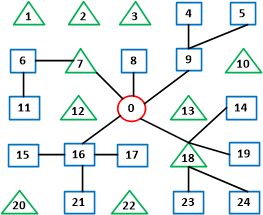
\includegraphics[width=0.6\linewidth]{images/graph}
		\caption{Mã hóa một cá thể}\label{fig:encode}
	\end{minipage}\hfill
	\begin{minipage}{0.2\textwidth}
		\centering
		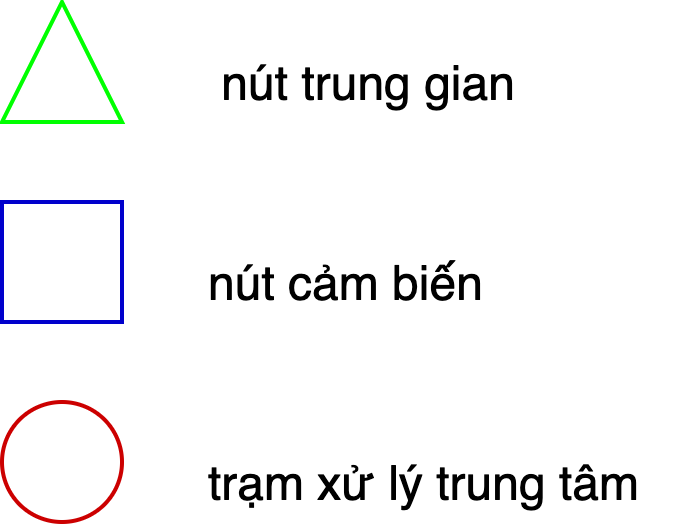
\includegraphics[width=1.2\linewidth]{images/diagram-note.png}
		\label{fig:note}
	\end{minipage}
\end{figure}

Hình \ref{fig:encode} mô tả mã hóa của một cá thể. Tập cạnh biểu diễn là: \{(0,7), (0,8), (0,9), (0,16), (7,6), (6,11), (9,4), (9,5), (16,15), (16, 17), (16,21), (18,14), (18,19), (18,23), (18,24)\}.


Việc mã hóa này đảm bảo một số tính chất quan trọng. Thứ nhất là tính bao quát, tất cả các lời giải khả dĩ đều có thể mã hóa được. Thứ hai là tính duy nhất, mỗi mã hóa chỉ có thể giải mã thành một lời giải duy nhất và ngược lại. Hơn thế, mã hóa sử dụng tập cạnh hỗ trợ thực hiện các nhiệm vụ khác như lai ghép, đột biến mà không cần chuyển đổi, do đó rút ngắn thời gian tính toán so với giải thuật đề xuất trong \cite{lu2014construction}.


Để xây dựng một cây từ tập E ban đầu, trước hết ta áp dụng Kruskal, nhưng thay vì với tập các cạnh được sắp xếp theo độ lớn tăng dần, ta sẽ sử dụng tập cạnh được xáo trộn để tăng tính đa dạng của toàn quần thể. Giải thuật Kruskal có thể dừng lại nếu tất cả các nút cảm biến đều đã được duyệt qua, và áp dụng một quy trình cắt tỉa các nốt thừa (các nốt lá không phải nút Steiner) để thu được một lời giải hợp lệ.


\subsection{Khởi tạo quần thể} \label{initialization}

Trong các giải thuật tiến hóa, khởi tạo quần thể là một bước vô cùng quan trọng. Có hai chiến lược thường được sử dụng để khởi tạo quần thể: tham lam hoặc ngẫu nhiên. Chiến lược tham lam được áp dụng với một trong tập các mục tiêu đang xem xét, với mục đích tăng tốc độ hội tụ và tìm được lời giải gần tối ưu theo mục tiêu có trọng số cao nhất. Chiến lược này tạo nên sự mất cân bằng và tính đa dạng cho toàn bộ quần thể khi các cá thể có xu hướng phân cực về mục tiêu có trọng số cao nhất. Chiến lược còn lại, ngẫu nhiên, được sử dụng khi muốn gia tăng phạm vi tìm kiếm của quần thể, đánh đổi lại là thời gian hội tụ sẽ lâu hơn.
Do các mục tiêu trong bài đều được đánh giá ngang nhau về mức độ quan trọng, giải thuật KGASL sử dụng chiến lược ngẫu nhiên trong toàn bộ quần thể. Để tạo sự ngẫu nhiên, từ tập cạnh lấy ra ban đầu của đồ thị, một số lượng ngẫu nhiên các cặp cạnh sẽ được lựa chọn để hoán đổi vị trí cho nhau, sau đó dùng tập cạnh mới này là đầu vào cho quy trình khởi tạo một cá thể đã trình bày ở trên.


\subsection{Toán tử lai ghép} \label{crossover}

Lai ghép trong giải thuật tiến hóa được sử dụng nhằm trao đổi thông tin giữa các cá thể trong một quần thể, tổng hợp các tính trạng trội để tạo ra các cá thể ở thế hệ sau tốt hơn thế hệ trước. Đầu tiên, tập các cạnh chung giữa hai cá thể được lựa chọn để thêm vào cá thể con. Tập cạnh này được coi như các "tính chất di truyền mạnh" cần được di truyền lại cho thế hệ sau. Để hoàn thiện cá thể con, tập thứ hai bao gồm các cạnh chỉ xuất hiện trong cá thể cha hoặc mẹ được xây dựng, sắp xếp theo thứ tự tăng dần của độ lớn và đưa vào cá thể con cho tới khi thu được một cây Steiner. Hình 3.2 mô tả quy trình lai ghép được áp dụng đối với một cặp cá thể cha và mẹ.

\begin{figure}[H]
	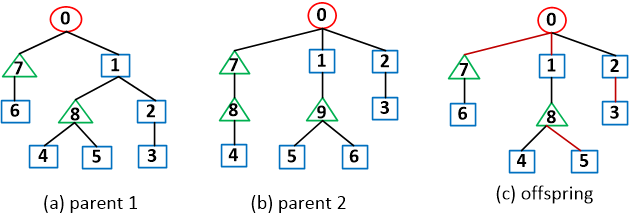
\includegraphics[scale=1.0]{images/crossover.png}
	\caption{Áp dụng toán tử lai ghép lên hai cá thể cha mẹ. Các cạnh xuất hiện trong cả cha và mẹ được tô đỏ ở cá thể con.} \label{fig:cross}
\end{figure}

\subsection{Toán tử đột biến} \label{mutation}

Đột biến được sử dụng như một cách giúp giải thuật thoát khỏi tối ưu hóa địa phương. Đây là vấn đề của quy trình khởi tạo và lai ghép. Khởi tạo ngẫu nhiên, tuy mục đích là bao phủ phạm vi tìm kiếm càng rộng càng tốt, nhưng do bản chất ngẫu nhiên mà không thực sự kiểm soát được độ bao phủ. Kết hợp với toán tử lai ghép làm toàn bộ quần thể có hàm mục tiêu hội tụ nhanh về một điểm cực tiểu/cực đại địa phương.
Đột biến hỗ trợ tìm kiếm ở những phạm vi mới, không nằm trong lân cận của vùng đang tìm kiếm. Tuy nhiên cần lựa chọn tỉ lệ đột biến một cách hợp lý, vì quy trình tìm kiếm cần càng rộng càng tốt ở những thế hệ đầu, nhưng càng nhanh càng tốt ở những thế hệ sau. Tỉ lệ đột biến sẽ tỉ lệ nghịch với số thứ tự của thế hệ, thế hệ càng lớn thì càng ít cá thể được đột biến.
Toán tử đột biến trong giải thuật đề xuất bắt đầu với việc lựa chọn hai nút u và v. Giả sử, không mất tính tổng quát, nút có độ sâu lớn hơn là v. Ta xóa cạnh nối giữa v và nút cha của nó, sau đó nối u với v. Bây giờ u sẽ là cha của v trong cá thể mới. Quy trình này mang tới hai ưa điểm. Thứ nhất là sự toàn vẹn tính hợp lệ của cá thể khi chu trình chắc chắn sẽ không tồn tại. Thứ hai là các nút còn lại được giữ nguyên tính chất, không có gì cần thay đổi.

\begin{figure}[H]
	\centering
	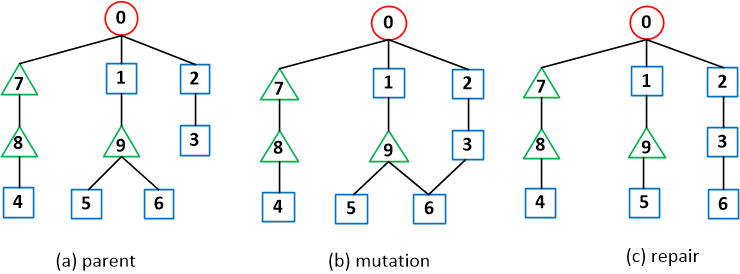
\includegraphics[scale=1.0]{images/mutation}
	\caption{Ví dụ về toán tử đột biến}\label{fig:mutation}
\end{figure}

\section{Giải thuật di truyền sắp xếp không trội}
\subsection{Cơ sở lý thuyết}
Một số khái niệm được sử dụng trong giải thuật di truyền sắp xếp không trội nói riêng và các bài toán tối ưu đa mục tiêu nói chung.
\begin{itemize}
	\item Lời giải trội: Với bài toán tối ưu đa mục tiêu, lời giải A được gọi là trội hơn lời giải B (kí hiệu là $A \prec B$) nếu tất cả các mục tiêu trong A có kết quả tốt hơn mục tiêu trong B.
	\item Lời giải không trội: Một lời giải được gọi là không trội nếu không tồn tại bất cứ lời giải nào trội hơn trong tập các lời giải.
	\item Biên pareto: Tập các lời giải không trội.
	\item Khoảng cách quần thể: Hệ số để hình thành đường bao giữa các lời giải không trội. Theo giải thích hình học, mỗi lời giải không trội được thể hiện là một điểm trên mặt phẳng, và khoảng cách quần thể được tính dựa trên ước lượng khoảng cách với hai điểm liền kề (các lời giải ở đầu mút sẽ có khoảng cách quần thể là vô cùng). Phép tính toán khoảng cách quần thể được trình bày trong mã giả \ref{alg:crownding_distance}
	\item Hạng: Hạng của mỗi lời giải được tính dựa trên số lượng lời giải trội hơn. Hạng càng nhỏ thì lời giải càng tốt (càng bị ít lời giải khác trội hơn).
	\item Toán tử so sánh: Khi sắp xếp các lời giải trong \gls{NSGA-II}, lời giải A tốt hơn lời giải B nếu $A_{rank} < B_{rank}$, nếu $A_{rank} = B_{rank}$ thì khoảng cách quần thể của A lớn hơn khoảng cách quần thể của B. Toán tử so sánh kí hiệu là $<$.
\end{itemize}
\subsection{Áp dụng cho bài toán tối ưu đa mục tiêu}
Giải thuật di truyền sắp xếp không trội được trình bày trong mã giả \ref{alg:nsga_ii}.

\begin{algorithm}[H]
	\caption{Giải thuật di truyền sắp xếp không trội}\label{alg:nsga_ii}
	\begin{algorithmic}[1]
		\Require Đồ thị không hoàn chỉnh vô hướng G=(V,E) với nút gốc $v_0 \in V$
		\Ensure Tập các cây Steiner trên biên Pareto
		\State Sinh n cá thể của quần thể $P_0$
		\For{cá thể $i \in P_0$}{ \\
			\begin{itemize}
				\item Thực hiện giải thuật Kruskal trên tập các cạnh đã xáo trộn để tạo thành một cây;
				\item Thực hiện quy trình sửa chữa để thu được cây Steiner;
				\item Tính toán hàm phạt của $i$;
			\end{itemize}
		}
		\EndFor
		\State $t\leftarrow 0$
		\While{điều kiện dừng chưa thỏa mãn}{
			\begin{itemize}
				\item $Q_t \leftarrow$ Thực hiện lai ghép và đột biến trên $P_t$;
				\item $R_t \leftarrow Q_t \cup P_t$;
				\item $F \leftarrow$ Thực hiện sắp xếp nhanh trên $R_t$ (mã giả \ref{alg:fast_non_dominated_sort});
				\item $P_t+1 \leftarrow$ Lựa chọn quần thể cho thế hệ t+1 (mã giả \ref{alg:select_parents});
				\item $t \leftarrow t+1$;
			\end{itemize}
		}
		\EndWhile
	\end{algorithmic}
\end{algorithm}

\begin{algorithm}[H]
	\caption{Quy trình sắp xếp nhanh cho \gls{NSGA-II}}\label{alg:fast_non_dominated_sort}
	\begin{algorithmic}[1]
		\Require Tập các cây Steiner (danh sách các cá thể ở thế hệ hiện tại).
		\Ensure Danh sách F của danh sách các cá thể, các phần tử thuộc cùng danh sách $F_i$ sẽ có hạng là i.
		\State F $\leftarrow$ [[]]
		\For{$p \in P$}
			\State $S_p \leftarrow []$ (tập các cá thể mà $p_i$ trội hơn)
			\State $n_p \leftarrow 0$ (số lượng các cá thể trội hơn $p_i$)
			\For{cá thể q của quần thể P}
				\If{$p \prec q$}
					\State $S_p \leftarrow S_p \cup q$
				\Else
					\State $n_p \leftarrow n_p + 1$
				\EndIf
			\EndFor
			
			\If{$n_p = 0$}
				\State $p_{rank} \leftarrow 0$
				\State $F[0] \leftarrow F[0] \cup p$
			\EndIf
		\EndFor
		
		\State i $\leftarrow$ 0
		\While {F[i] $\neq \emptyset$}
			\State Q $\leftarrow []$
			\For{$p \in F[i]$}
				\For{$q \in S_p$}
					$n_q \leftarrow n_q - 1$
					\If{$n_q = 0$}
						\State $q_{rank} = i+1$
						\State $Q \leftarrow Q \cup q$
					\EndIf
				\EndFor
			\EndFor
			\State $i \leftarrow i+1$
			\State $F[i] \leftarrow Q$
		\EndWhile
		
		
	\end{algorithmic}
\end{algorithm}

\begin{algorithm}[H]
	\caption{Phép lựa chọn quần thể cho \gls{NSGA-II}}
	\label{alg:select_parents}
	\begin{algorithmic}[1]
		\Require Danh sách F của danh sách các cá thể.
		\Ensure Tập các cá thể với kích thước bằng n, bằng kích thước thể ban đầu.
		\For{$F[i] \in F$}
			\State Tính toán khoảng cách quần thể cho danh sách F[i]
		\EndFor
		\State $P \leftarrow []$
		\State $last-front \leftarrow 0$
		\For{$F[i] \in F$}
			\If{$len(P) + len(F[i]) < n$}
				\For $p \in F[i]$
					$P \leftarrow P \cup p$
				\EndFor
				\State $last-front \leftarrow last_front+1$
			\EndIf
		\EndFor
		\State $remaining-size \leftarrow n - len(P)$
		\If{$remaining-size > 0$}
			\State $sort(F[last-front], <)$
			\State $P \leftarrow P \cup F[last-front][:remaining-size+1]$
		\EndIf
	\end{algorithmic}
\end{algorithm}

\begin{algorithm}[H]
	\caption{Phép tính toán khoảng cách quần thể cho \gls{NSGA-II}}
	\label{alg:crownding_distance}
	\begin{algorithmic}[1]
		\Require Tập các cá thể ở danh sách $F_i$ (các cá thể có cùng hạng là i).
		\For{$j \in len(F_i)$}
			\State $dist_j \leftarrow 0$
		\EndFor
		\For{mục tiêu thứ i trong m mục tiêu}
			\State $z_{max} \leftarrow MIN$ (giá trị lớn nhất của mục tiêu thứ i)
			\State $z_{min} \leftarrow MAX$ (giá trị nhỏ nhất của mục tiêu thứ i)
			\For{$p \in F_i$}
				\State $z_{max} = max(z_{max}, p_i)$
				\State $z_{min} = min(z_{min}, p_i)$
			\EndFor
			\State $dist_0 \leftarrow MAX$
			\State $dist_{len(F[i])-1} \leftarrow MAX$
			\For{$j \in [1,len(F[i])-2]$}
				\State $dist_j \leftarrow dist_j + (dist_{j+1} - dist_{j-1})/(z_{max} - z_{min})$
			\EndFor
		\EndFor
	\end{algorithmic}
\end{algorithm}
\section{Hàm phạt}
Có hai cách để đánh giá giữa các lời giải khác nhau trong bài toán đa mục tiêu: thực hiện chuẩn hóa các mục tiêu để đưa về một hàm số duy nhất hoặc sử dụng biên Pareto. Cả hai cách này đều có nhược điểm. Cách thứ nhất thì trọng số đánh giá của từng mục tiêu thường không được đánh giá một cách chính xác, còn cách thứ hai thì chỉ tập trung vào việc phân tích sự khác nhau giữa các phương án trội và bị trội, sự khác nhau giữa các lời giải trên cùng biên Pareto không được đề cập cụ thể. 


Một cách đánh giá là tổng hợp từ hai cách trên được đề xuất trong \ref{lu2014construction}. Trong đó, giá trị Pareto được sử dụng như một giá trị phạt để phân biệt giữa các lời giải trội và bị trội. Còn giá trị của các mục tiêu sẽ được chuẩn hóa với các giá trị cực đại và cực tiểu của từng mục tiêu trong suốt quá trình tính toán.

\begin{equation}\label{eq:fitness}
fitness (x) = \frac{1}{\sum_{i=1}^4 \overline{f_i}(x) + Pen(x)}
\end{equation}

với
\begin{equation}\label{eq:newObjective}
\overline{f_i}(x) = \frac{f_i(x) - t^{min}_i}{t^{max}_i - t^{min}_i}
\end{equation}
trong đó $t^{max}_i$ và $t^{min}_i$ đại diện cho giá trị cực đại và cực tiểu của mục tiêu thứ $i$. $f_i(x)$ là giá trị của mục tiêu thứ $i$ được đề cập ở chương trước.

và
\begin{equation}
Pen(x) = \begin{cases}
0 & \text{$x$ nằm trên biên Pareto,}\\
1 & \text{trong trường hợp ngược lại}\\
\end{cases}
\end{equation}

Ở phương trình \ref{eq:fitness}, giá trị càng cao càng thể hiện mức độ tối ưu của lời giải.


\chapter{Thực nghiệm}
\section{Mô tả dữ liệu}
Kết quả thực nghiệm được tiến hành trên tập dữ liệu mô phỏng địa hình các tỉnh thành Việt Nam \cite{tam2018improving}. Tập dữ liệu có tất cả 12- bộ dữ liệu, bao gồm 10 địa hình được đánh thứ tự từ T1 tới T10, mô tả ngắn gọn trong \ref{tab:terrain}, bán kính cảm biến của các nút trong mỗi bộ dữ liệu nhận 1 trong 4 giá trị: 25, 30, 45, hoặc 50 mét, các nút cảm biến được phân bố trên các địa hình theo 1 trong 3 phân phối: phân phối chuẩn, phân phối đều, hoặc phân phối gamma. Dữ liệu được xây dựng theo chuẩn Digital Elevation Model.

\begin{table}[H]
	\caption{Tính chất các địa hình}\label{tab:terrain}
	\resizebox{1.0\textwidth}{!}{
		\begin{tabular}{|c|l|l|}
			\hline
			Địa hình 		& Địa điểm    		& Tính chất \\
			\hline
			T1      		   & Hồ Chí Minh 	& Thành phố nhiều tòa nhà đa dạng về độ cao, không có đồi núi, sông \\ \hline
			T2      		   & Vũng Tàu   	 & Thành phố nhiều tòa nhà với độ cao cân đối, có đồi núi, và một vùng biển nằm về một hướng \\ \hline
			T3      		   & Phú Quốc    	& Vùng đảo có đồi núi với độ cao thấp khác nhau, vùng biển là chính \\ \hline
			T4      		   & Đồng Tháp   	& Vùng đồng bằng ít nhà cửa, sông, kênh rạch nhiều, không đồi núi \\ \hline
			T5      		   & Vĩnh Long  	 & Ít nhà cửa, không đồi núi, kênh rạch nhiều, đặc biệt có dòng sông lớn Mekong \\ \hline
			T6      		   & Lâm Đồng    	& Vùng đồi núi nhiều, ít nhà cửa, có núi cao, có sông xen kẽ \\ \hline
			T7      		   & Cao Nguyên    & Vùng có nhiều đồi núi có độ cao tăng dần, ít nhà cửa, không sông hồ \\ \hline
			T8      		   & Đà Nẵng     	 & Vùng ít nhà cửa, núi cao tiếp giáp vùng biển \\ \hline
			T9      		   & Hà Nội      	   & Vùng nhiều nhà cao, có ao hồ \\ \hline
			T10     		   & Hạ Long     	 & Vùng biển có nhiều đảo nhỏ độ cao khác nhau, không có nhà \\ \hline
	\end{tabular}}
\end{table}

\section{Tham số cố định}
Các tham số cố định được sử dụng trong quá trình thực nghiệm được đề cập trong bảng \ref{tab:1} và \ref{tab:2}.

\begin{table}[H]
	\caption{Tham số sử dụng trong mô phỏng địa hình}\label{tab:1}
	\centering
	\begin{tabularx}{0.6\textwidth} {X l}
		\hline
		\textbf{Tham số}              & \textbf{Giá trị}    \\ \hline
		Kích thước địa hình        & $500 \times 500 m^2$  \\
		Số lượng nút cảm biến         & 100      \\                
		Số lượng nút trung gian & 100         \\         
		Bán kính cảm biến & 25-50 m \\ \hline
	\end{tabularx}
\end{table}

\begin{table}[H]
	\caption{Tham số cài đặt trong các giải thuật}\label{tab:2}
	\centering
	\begin{tabularx}{0.6\textwidth} {X l}
		\hline
		\textbf{Tham số}              & \textbf{Giá trị}    \\ \hline
		Kích thước quần thể    & 50  \\ 
		Tỉ lệ lai ghép & 0.8    \\
		Tỉ lệ đột biến & 0.05        \\                
		Số lượng thế hệ & 150 \\     \hline  
	\end{tabularx}
\end{table}

Các giải thuật được cài đặt bằng Python3 và chạy trên Intel Core i5-5200u 2.20 GHz, 8GB RAM, hệ điều hành Ubunutu 16.04.

\section{Kết quả thực nghiệm của \gls{GA} và \gls{JPSO} trên các phân phối khác nhau}
Dưới đây là kết quả thực nghiệm của giải thuật \gls{GA} và \gls{JPSO} nêu trong \cite{lu2014construction} khi áp dụng trên ba phân phối: phân phối chuẩn, phân phối đều và phân phối Gamma, với bán kính giao tiếp của các cảm biến đều là 30 mét.

%\begin{figure}[!hbt]
%	\centering
%	\caption{Phân phối gamma}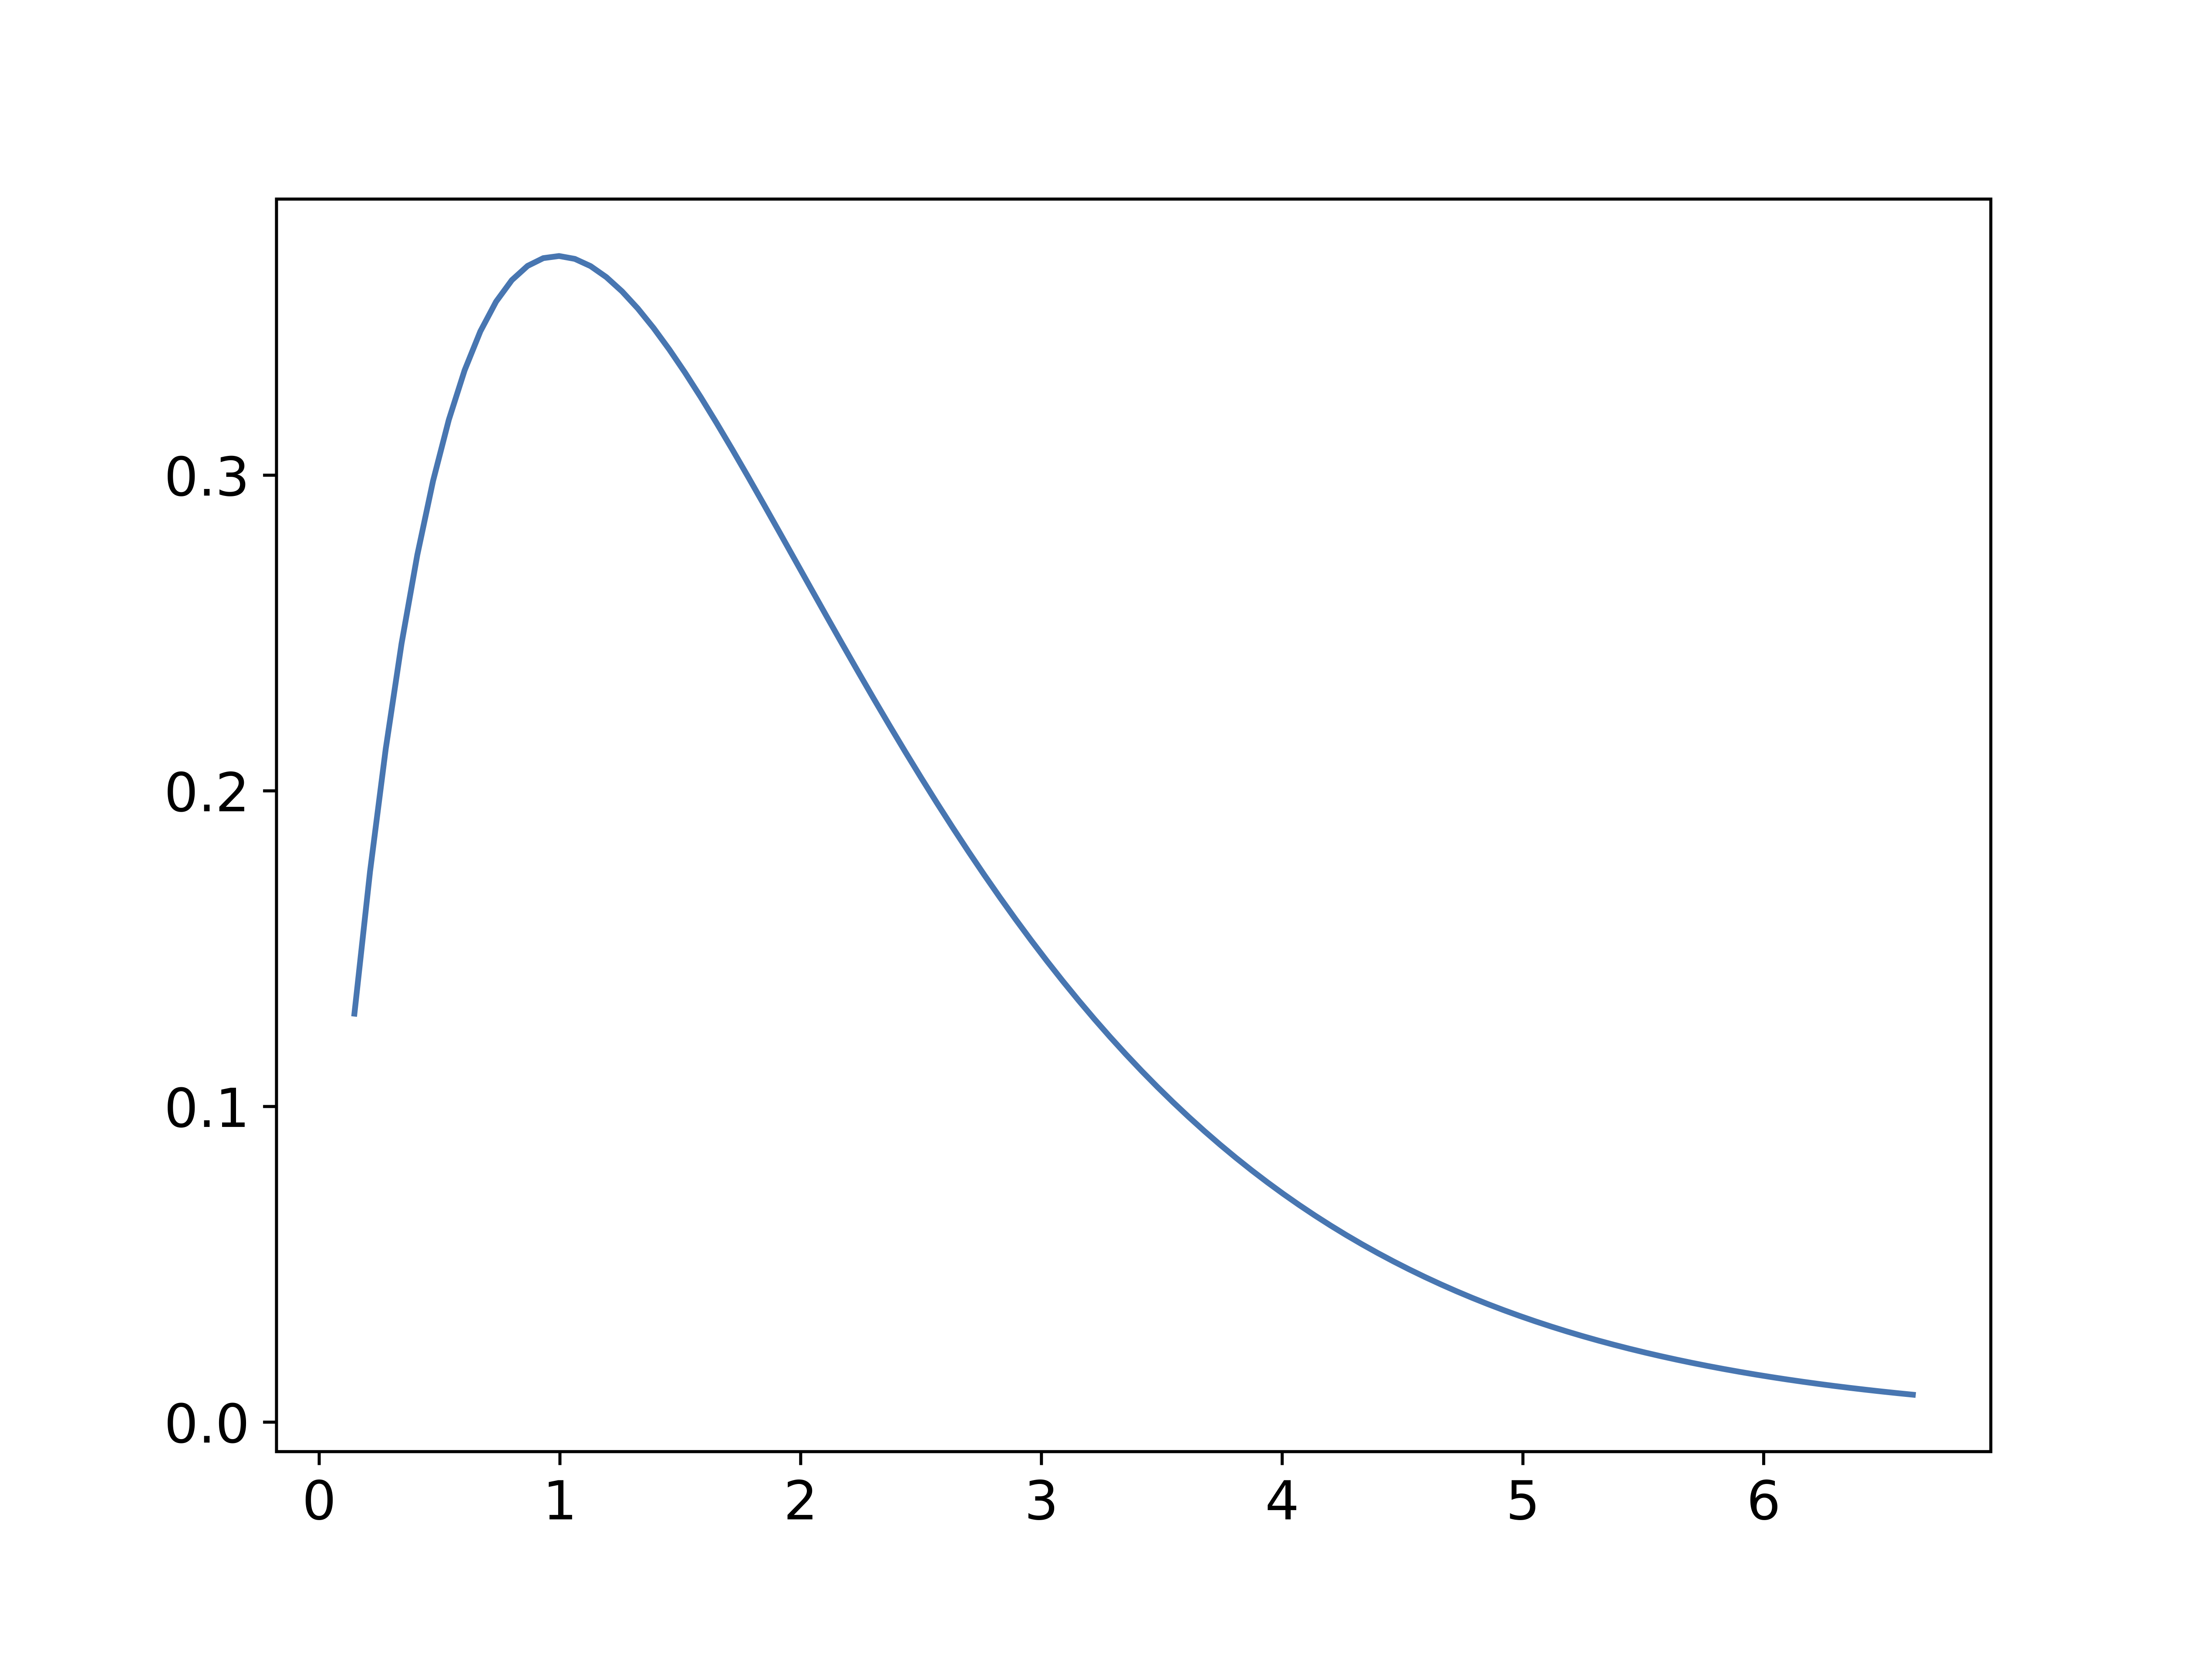
\includegraphics[width=0.15\textwidth , height=0.15 \textheight]{images/gamma.png}
%	\caption{Phân phối chuẩn}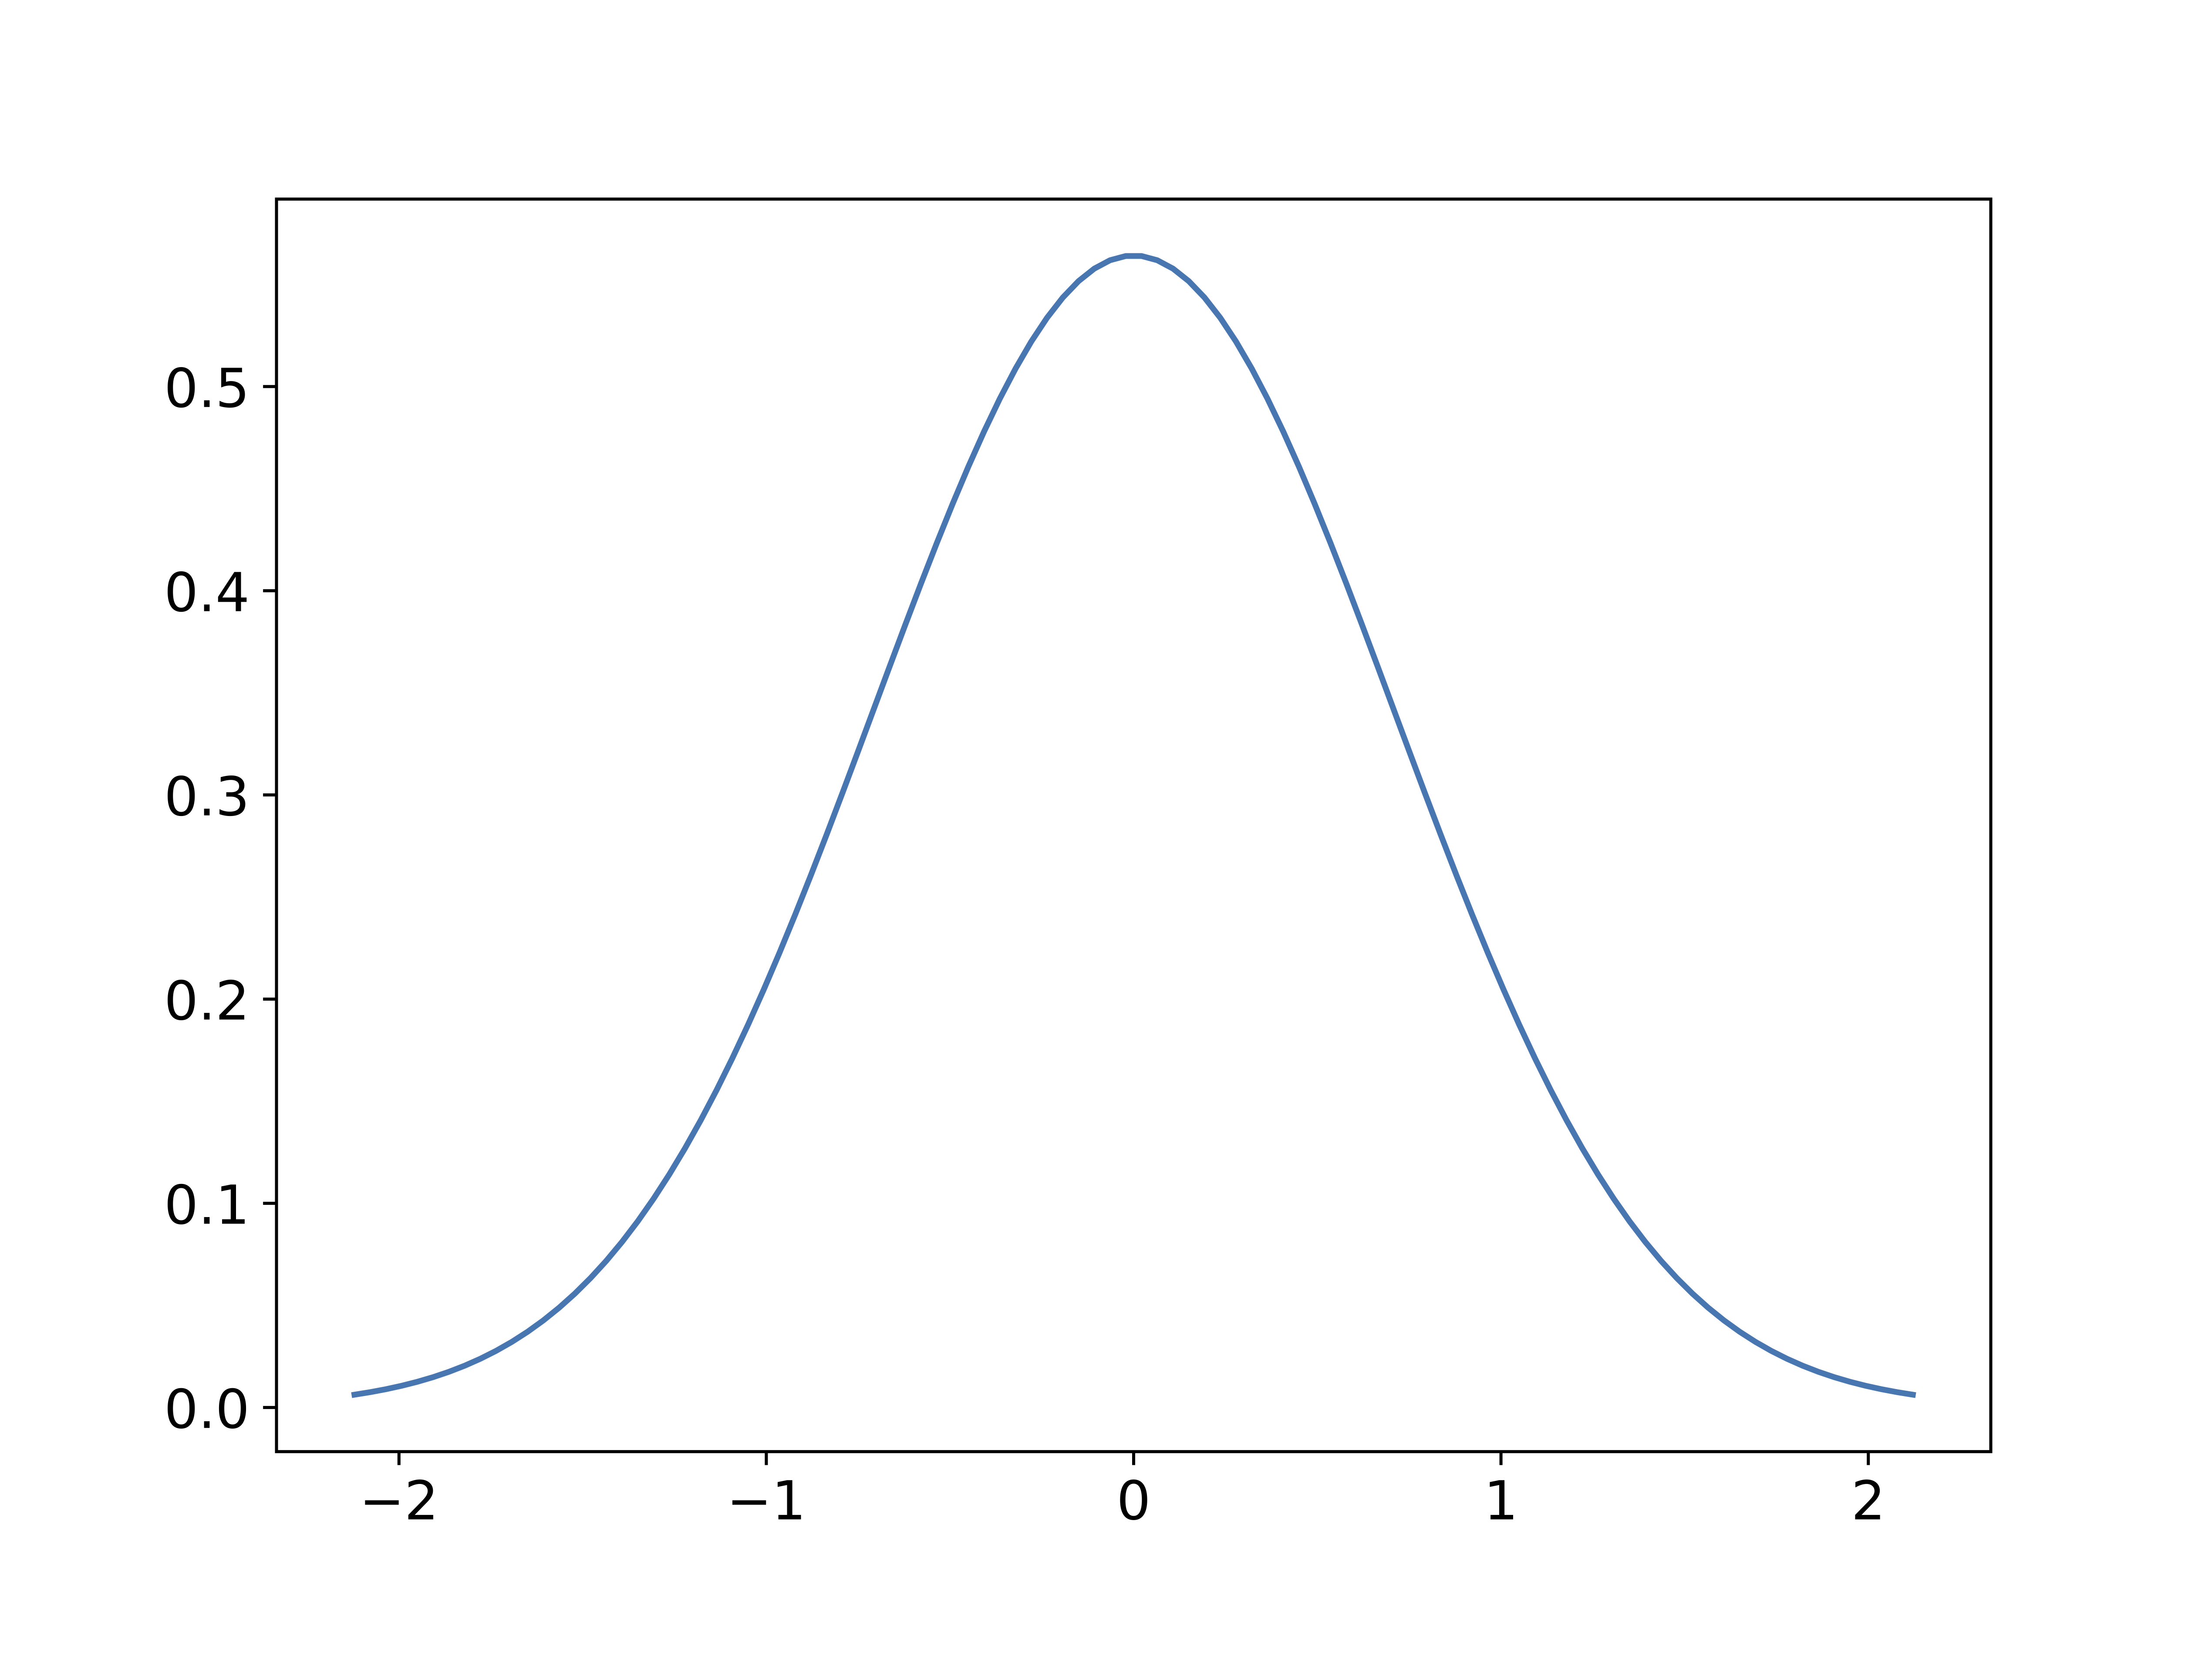
\includegraphics[width=0.15\textwidth , height=0.15 \textheight]{images/normal.png}
%	\caption{Phân phối đều}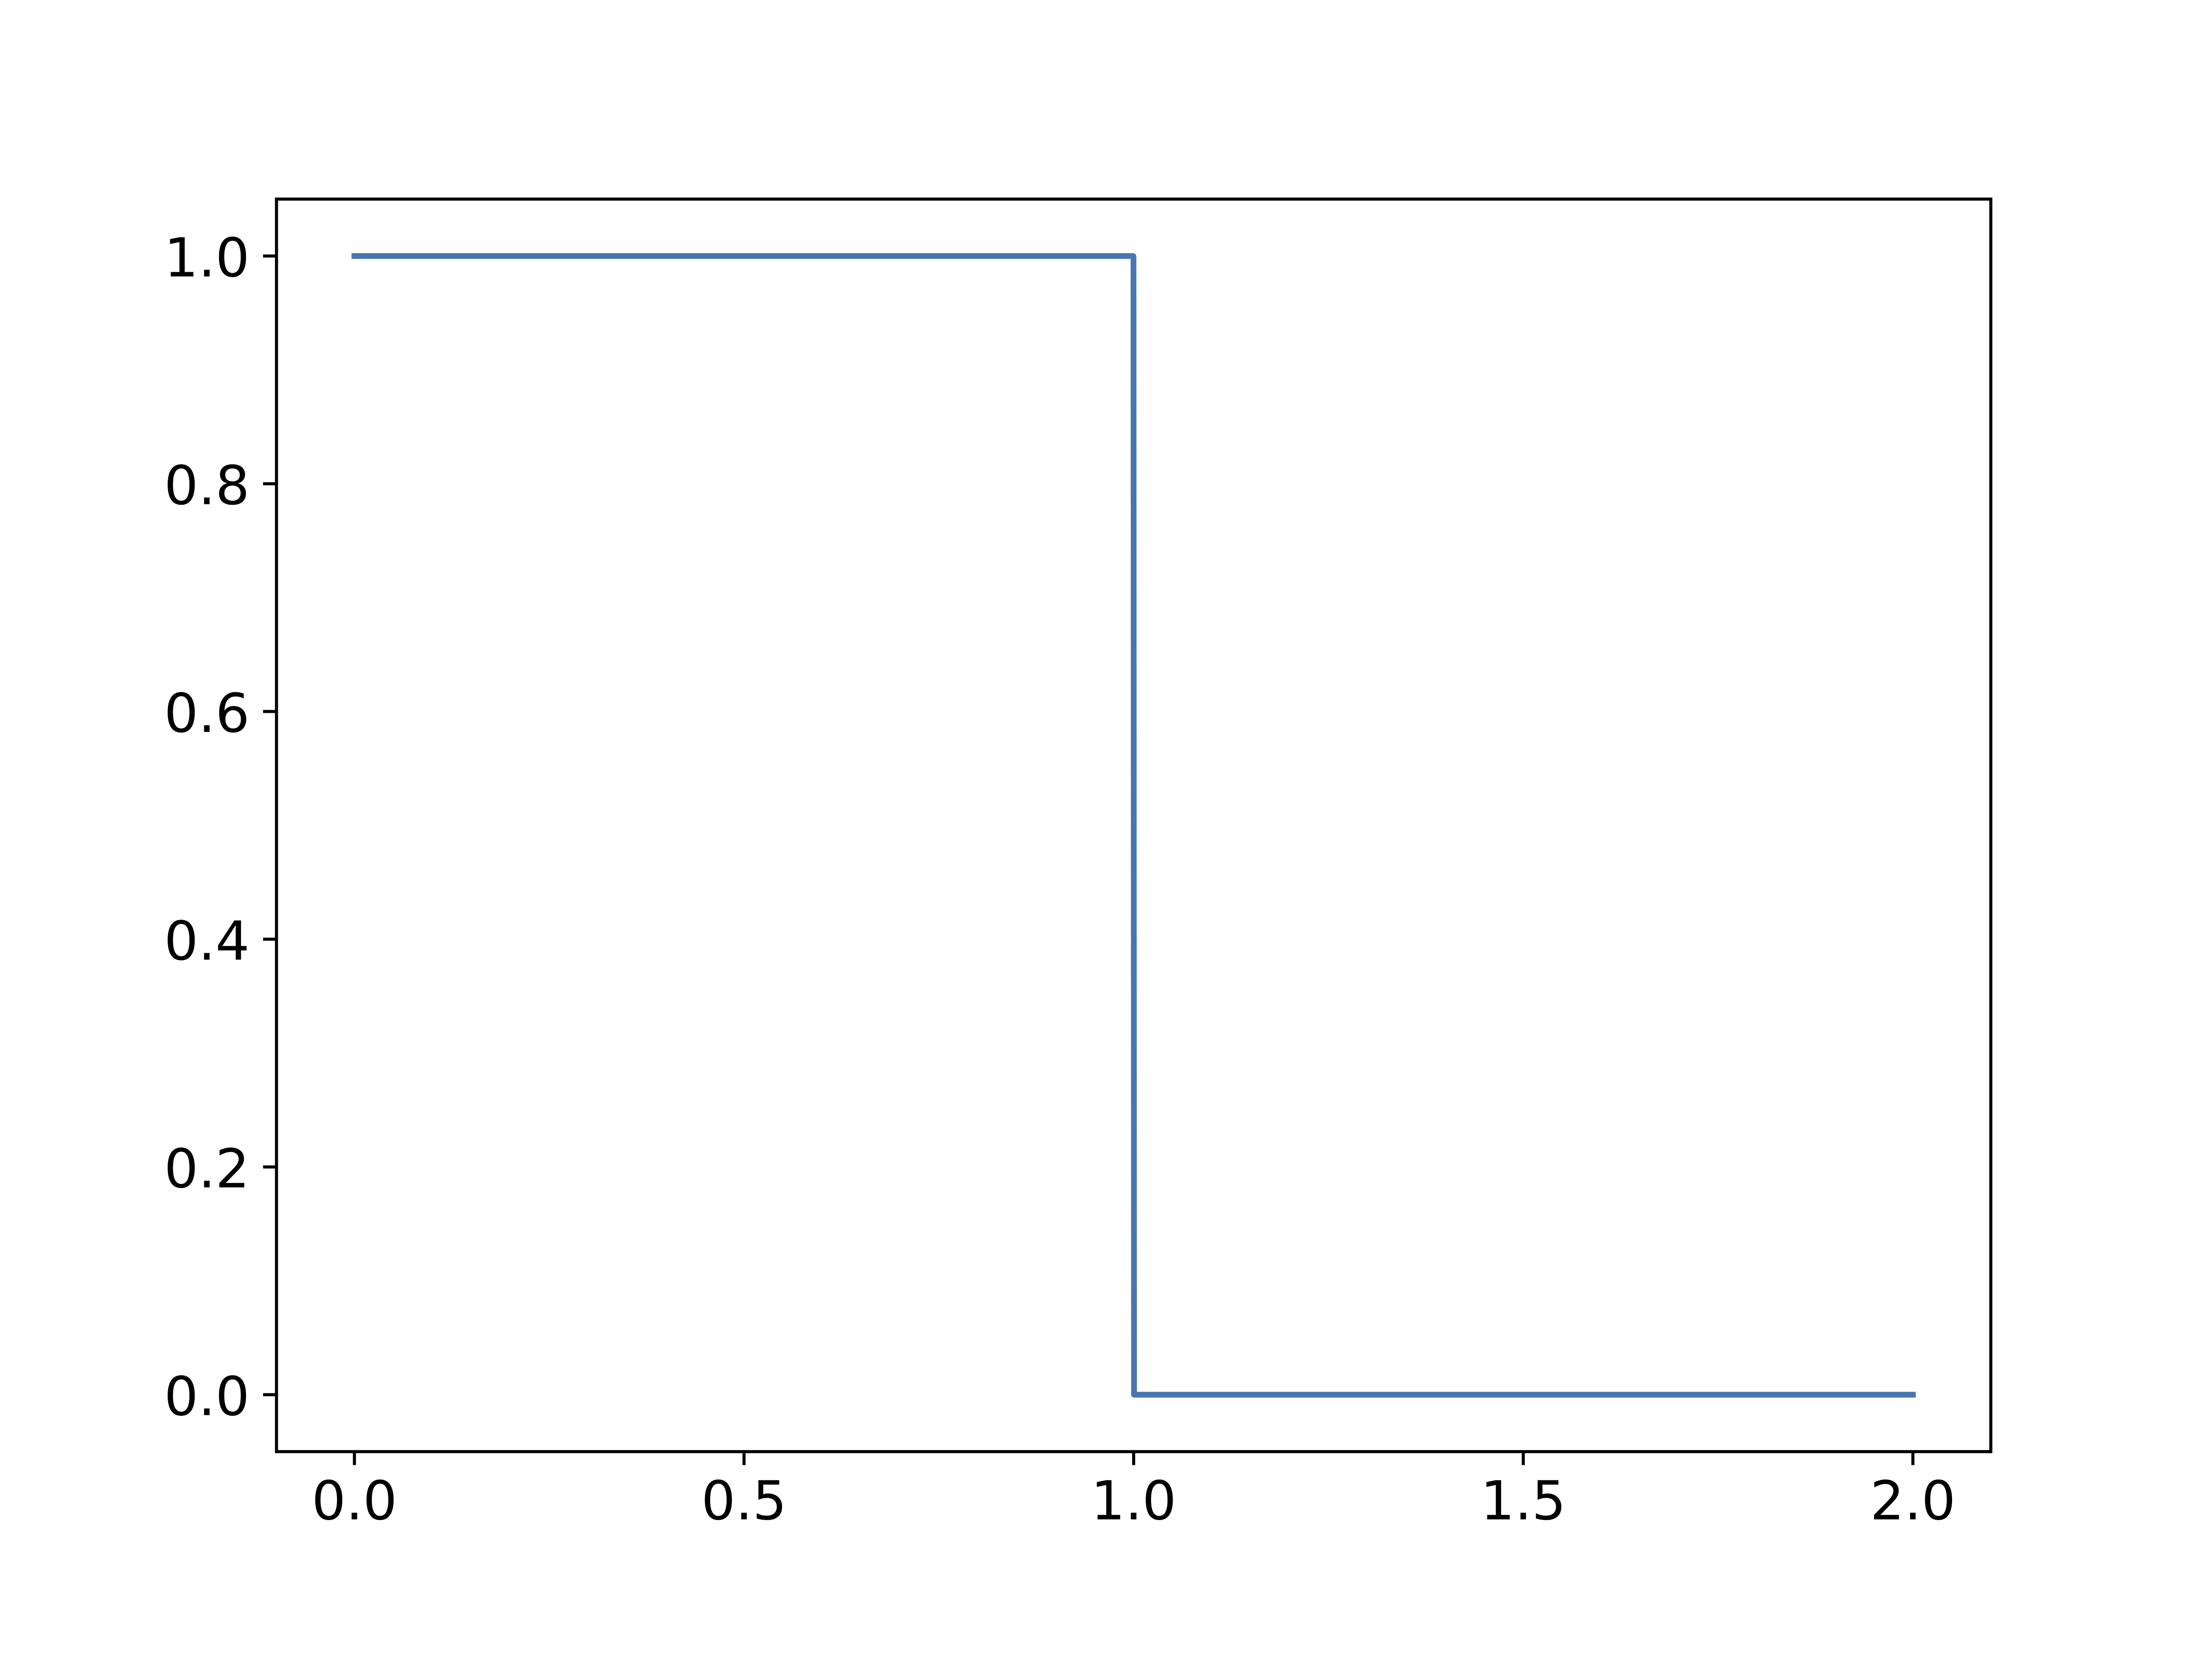
\includegraphics[width=0.15\textwidth , height=0.15 \textheight]{images/uniform.png}
%	\caption{Kết quả thực nghiệm trên các phân phối khác nhau.}\label{fig:dis}
%\end{figure}


\begin{figure}[H]
	\centering
	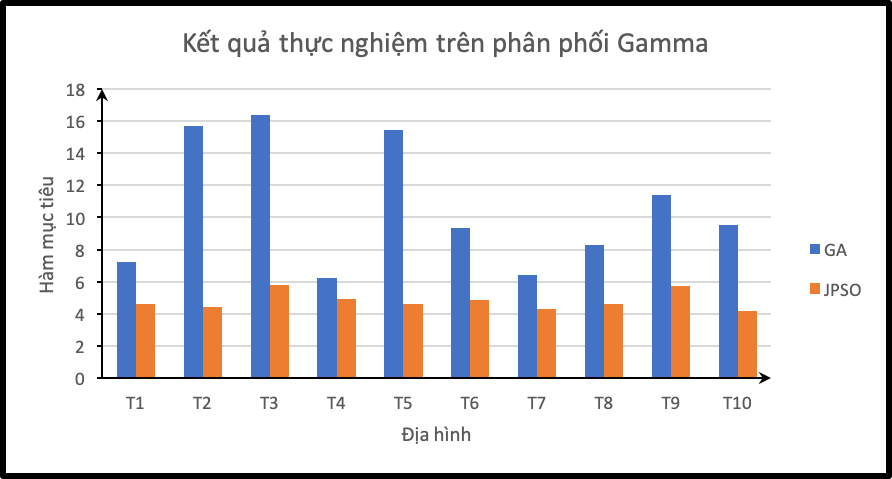
\includegraphics[width=0.7\textwidth]{images/medium_gamma.png}
	\caption{Giá trị trung bình hàm mục tiêu của \gls{GA} và \gls{JPSO} trên phân phối Gamma.} \label{fig:medium_gamma}
\end{figure}

\begin{figure}[H]
	\centering
	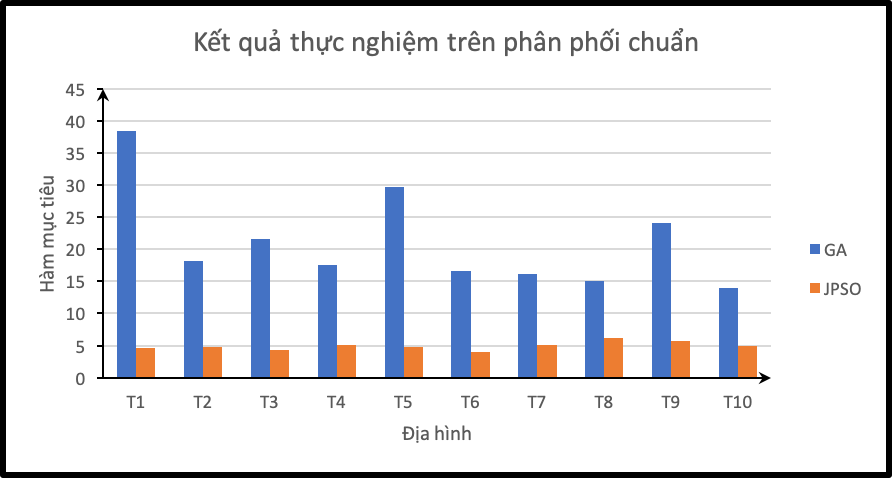
\includegraphics[width=0.7\textwidth]{images/medium_normal.png}
	\caption{Giá trị trung bình hàm mục tiêu của \gls{GA} và \gls{JPSO} trên phân phối chuẩn.} \label{fig:medium_norm}
\end{figure}

\begin{figure}[H]
	\centering
	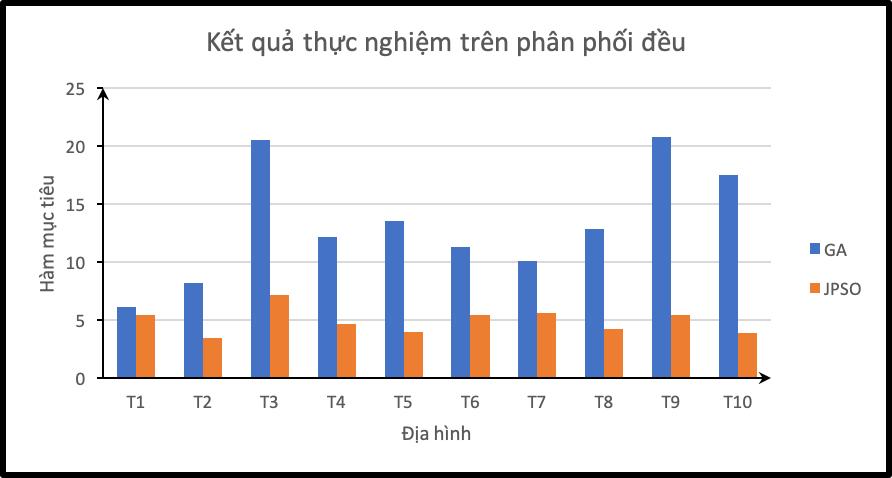
\includegraphics[width=0.7\textwidth]{images/medium_uniform.png}
	\caption{Giá trị trung bình hàm mục tiêu của \gls{GA} và \gls{JPSO} trên phân phối đều.} \label{fig:medium_uniform}
\end{figure}


Nhận thấy trên cả ba phân phối, giá trị hàm mục tiêu thu được từ \gls{GA} luôn tốt hơn \gls{JPSO}, với sự khác biệt được thể hiện rõ nhất ở phân phối chuẩn. Một điều đáng lưu ý là kết quả của \gls{JPSO} không có sự sai khác quá nhiều giữa các địa hình, cho thấy thuật toán có khả năng đã rơi vào tối ưu lân cận trên bộ dữ liệu thực nghiệm. Sự khác biệt nhiều nhất giữa hai giải thuật được thể hiện ở phân phối chuẩn, với các nút cảm biến được bố trí gần hơn với trạm xử lý trung tâm so với hai phân phối còn lại.

\pagebreak
\subsection{Tổng hợp kết quả thực nghiệm của \gls{GA} và \gls{JPSO}}

%\begin{figure}[htp]
%	\centering
%	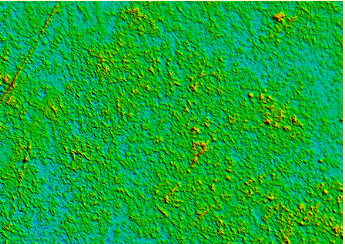
\includegraphics[width=15mm]{images/t1.png}
%	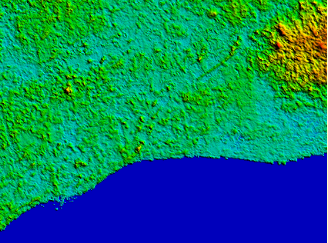
\includegraphics[width=15mm]{images/t2.png}
%	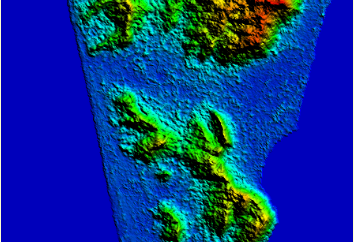
\includegraphics[width=15mm]{images/t3.png}
%	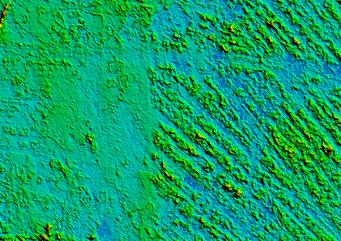
\includegraphics[width=15mm]{images/t4.png}
%	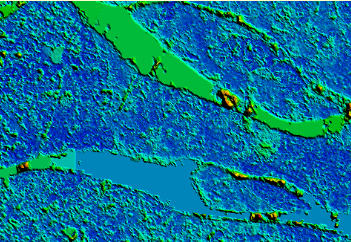
\includegraphics[width=15mm]{images/t5.png}
%	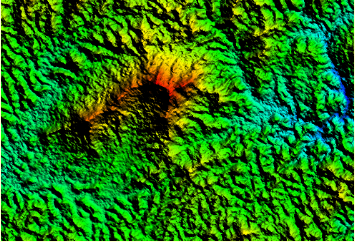
\includegraphics[width=15mm]{images/t6.png}
%	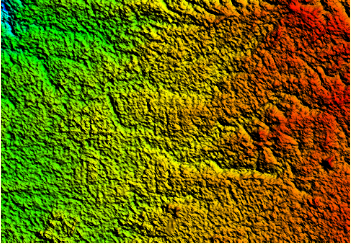
\includegraphics[width=15mm]{images/t7.png}
%	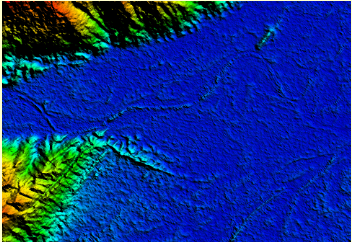
\includegraphics[width=15mm]{images/t8.png}
%	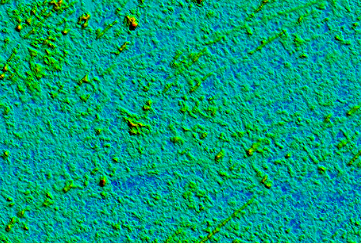
\includegraphics[width=15mm]{images/t9.png}
%	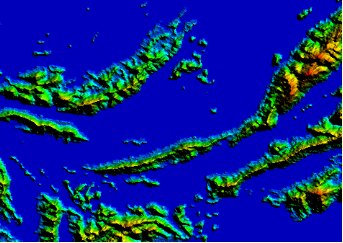
\includegraphics[width=15mm]{images/10.png}
%	\caption{Độ cao của các địa hình trong tập dữ liệu.}\label{fig:terrain}
%\end{figure}

Bảng \ref{fig:exp_table} tổng hợp kết quả thực nghiệm của \gls{GA} và \gls{JPSO} trên 120 bộ dữ liệu, bao gồm 10 loại địa hình, 3 loại phân phối và 4 loại bán kính khác nhau.

\begin{center}
\begin{table*}[htb]
	\centering
	\caption{Bảng tổng hợp giá trị hàm mục tiêu.\label{fig:exp_table}}
\begin{adjustwidth}{-1.8cm}{}
\begin{tabular}{|l|l|l|l|l|l|l|l|l|l|}
	\hline
	\multirow{2}{*}{Phân phối} 
	& \multirow{2}{*}{Địa hình} 
	& \multicolumn{2}{c|}{r=25} & \multicolumn{2}{c|}{r=30} 
	& \multicolumn{2}{c|}{r=45} & \multicolumn{2}{c|}{r=50} \\ \cline{3-10} 
	&    &GA &JPSO  &GA &JPSO &GA &JPSO &GA &JPSO \\ \hline
	\multirow{10}{*}{Phân phối Gamma}   
	&T1	&8.83	&4.37	&7.21	&4.61	&10.28	&5.49	&17.18	&4.95	\\
	&T2	&7.44	&5.76	&15.68	&4.43	&11.13	&4.67	&8.05	&5.87	\\
	&T3	&9.31	&4.92	&16.41	&5.81	&29.86	&11.15	&20.66	&4.49	\\
	&T4	&19.69	&3.51	&6.22	&4.93	&5.17	&5.4	&28.81	&7.31	\\
	&T5	&9.55	&5.85	&15.44	&4.61	&6.63	&4.01	&6.58	&5.49	\\
	&T6	&9.4	&5.8	&9.36	&4.88	&14.39	&4.43	&17.85	&3.78	\\
	&T7	&6.57	&5.63	&6.45	&4.31	&10.99	&4.31	&9.96	&4.92	\\
	&T8	&7.87	&7.94	&8.31	&4.6	&26.15	&4.44	&12.11	&5.28	\\
	&T9	&15.81	&5.15	&11.38	&5.72	&7.25	&8.23	&8.01	&6.53	\\
	&T10	&13.71	&5.17	&9.52	&4.18	&9.54	&5.35	&8.39	&5.27	\\ \hline
	\multirow{10}{*}{Phân phối chuẩn}  
	&T1	&22.44	&7.44	&38.41	&4.57	&20.5	&4	&15.12	&4.28	\\
	&T2	&23.83	&5.27	&18.22	&4.76	&5.89	&6.86	&11.26	&3.42	\\
	&T3	&15.8	&4.85	&21.63	&4.26	&18.14	&7.3	&43.12	&4.4	\\
	&T4	&20.78	&5.05	&17.61	&5.15	&26.91	&4.02	&11.96	&3.77	\\
	&T5	&11.77	&7.31	&29.63	&4.86	&12.4	&3.34	&25.33	&4.94	\\
	&T6	&23.92	&5.38	&16.55	&3.96	&20.99	&4.67	&13.31	&5.52	\\
	&T7	&20.12	&4.84	&16.09	&5.07	&20.53	&6.67	&8.28	&6.85	\\
	&T8	&25.85	&4.44	&15	&6.18	&22.17	&5.45	&18.11	&4.42	\\
	&T9	&14.86	&6.13	&24.01	&5.67	&6.48	&3.52	&8.05	&3.72	\\
	&T10	&11.09	&4.29	&13.91	&4.92	&13.93	&5.27	&22.76	&4.68	\\ \hline
	\multirow{10}{*}{Phân phối đều}      
	&T1	&27.23	&5.02	&4.14	&5.37	&11.38	&6	&12.29	&4.49	\\
	&T2	&6.7	&5.65	&8.17	&3.43	&7.34	&3.97	&8.01	&4.81	\\
	&T3	&31.4	&5.5	&20.5	&7.11	&5.08	&3.64	&8.74	&4.27	\\
	&T4	&16.55	&4.34	&12.16	&4.66	&20.31	&5.31	&14.69	&4.14	\\
	&T5	&9.43	&4.18	&13.57	&3.95	&10.52	&4.53	&18.19	&4.15	\\
	&T6	&28.29	&5.01	&11.28	&5.4	&17.66	&3.95	&12.74	&5.83	\\
	&T7	&11.73	&6.15	&10.12	&5.55	&6.8	&6.1	&18.77	&3.86	\\
	&T8	&17.95	&4.97	&12.85	&4.18	&14.34	&5.02	&8.11	&6.06	\\
	&T9	&27.23	&5.23	&20.83	&5.45	&16.54	&5.53	&30.81	&3.93	\\
	&T10	&13.79	&6.86	&17.54	&3.82	&14.02	&4.18	&10.39	&5.49	\\ \hline
\end{tabular}
\end{adjustwidth}
\end{table*}
\end{center}

\subsection{Kết quả thực nghiệm của \gls{NSGA-II}}
Dưới đây là hình vẽ biên Pareto trên các bộ dữ liệu với phân phối khác nhau, bán kính các nút cảm biến đều là 30 mét.

\begin{itemize}
	\item Phân phối Gamma
	\begin{figure}[H]
		\begin{minipage}{0.5\textwidth}
			\centering
			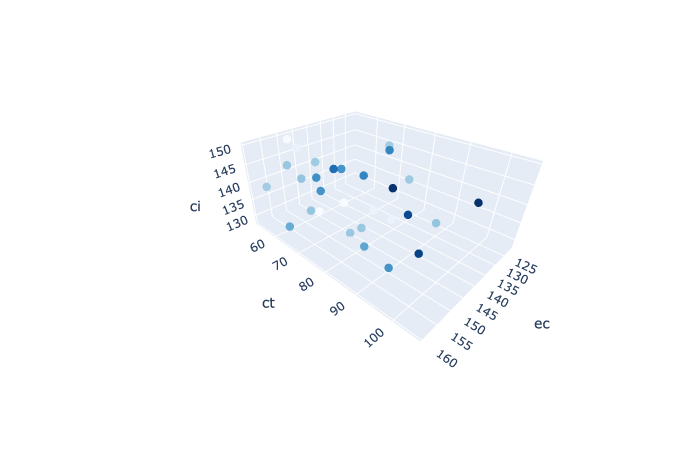
\includegraphics[width=1.2\linewidth]{images/ga-dem1.png}
			\caption{Gamma - T1}\label{fig:nsga-ii-ga-dem1}
		\end{minipage}\hfill
		\begin{minipage}{0.5\textwidth}
			\centering
			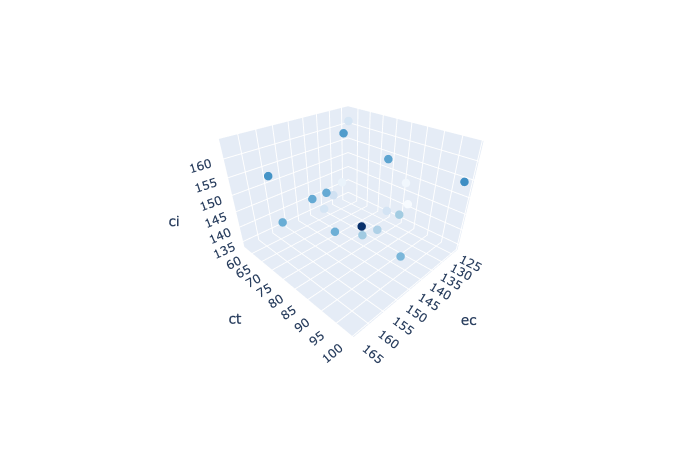
\includegraphics[width=1.2\linewidth]{images/ga-dem2.png}
			\caption{Gamma - T2}\label{fig:nsga-ii-ga-dem2}
		\end{minipage}
	\end{figure}
	
	\begin{figure}[H]
		\begin{minipage}{0.5\textwidth}
			\centering
			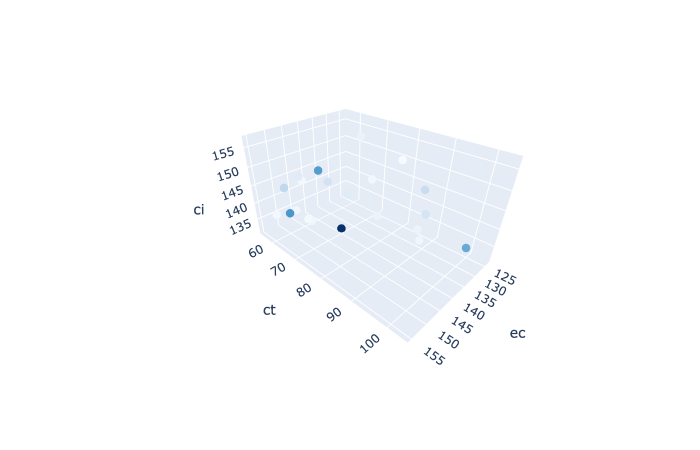
\includegraphics[width=1.2\linewidth]{images/ga-dem3.png}
			\caption{Gamma - T3}\label{fig:nsga-ii-ga-dem3}
		\end{minipage}\hfill
		\begin{minipage}{0.5\textwidth}
			\centering
			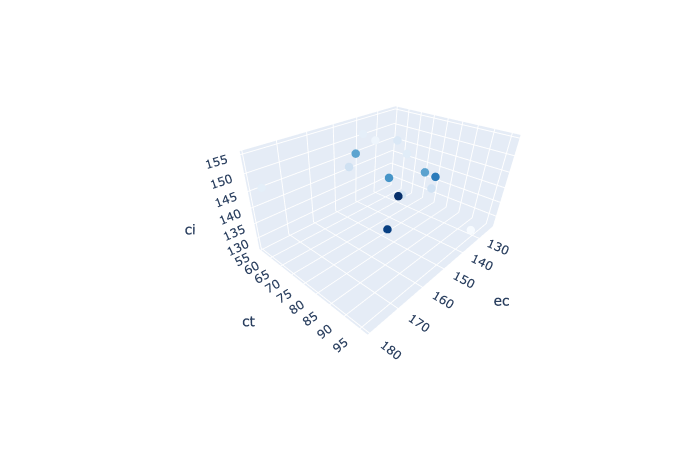
\includegraphics[width=1.2\linewidth]{images/ga-dem4.png}
			\caption{Gamma - T4}\label{fig:nsga-ii-ga-dem4}
		\end{minipage}
	\end{figure}

	\begin{figure}[H]
		\begin{minipage}{0.5\textwidth}
			\centering
			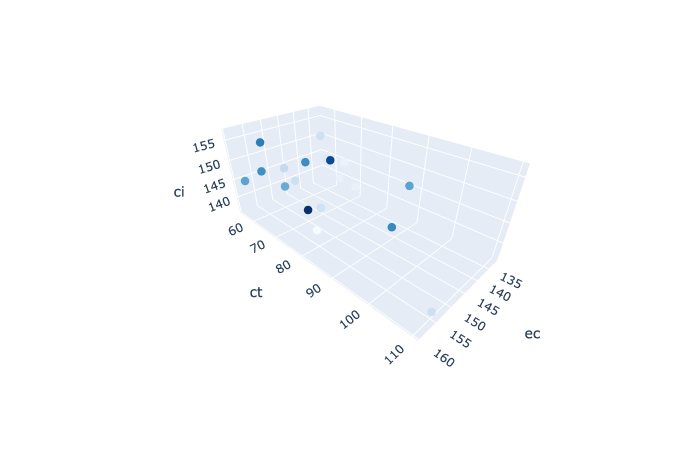
\includegraphics[width=1.2\linewidth]{images/ga-dem5.png}
			\caption{Gamma - T5}\label{fig:nsga-ii-ga-dem5}
		\end{minipage}\hfill
		\begin{minipage}{0.5\textwidth}
			\centering
			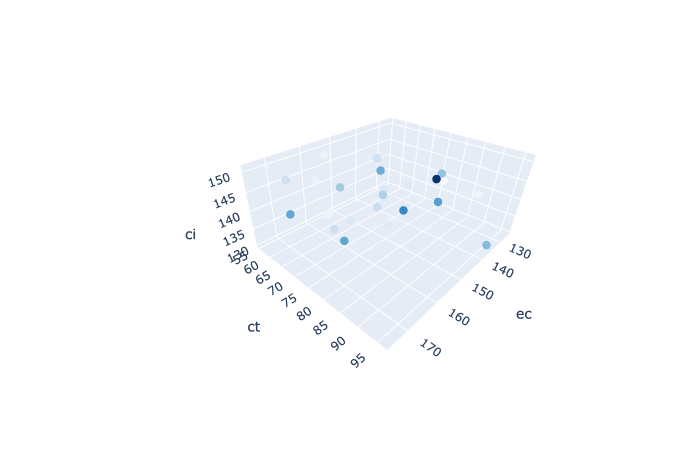
\includegraphics[width=1.2\linewidth]{images/ga-dem6.png}
			\caption{Gamma - T6}\label{fig:nsga-ii-ga-dem6}
		\end{minipage}
	\end{figure}

	\begin{figure}[H]
		\begin{minipage}{0.5\textwidth}
			\centering
			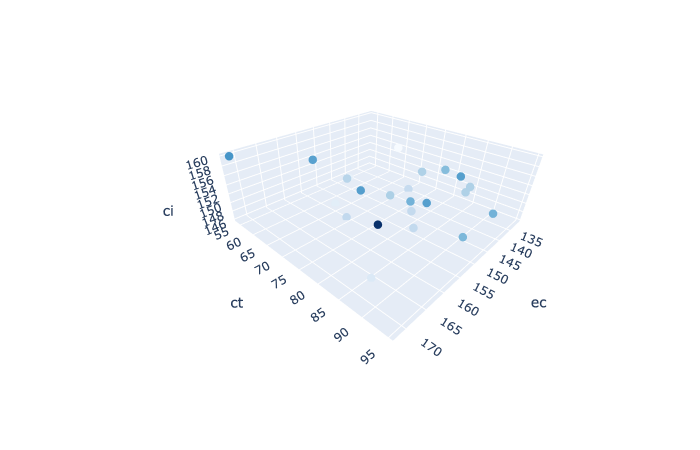
\includegraphics[width=1.2\linewidth]{images/ga-dem7.png}
			\caption{Gamma - T7}\label{fig:nsga-ii-ga-dem7}
		\end{minipage}\hfill
		\begin{minipage}{0.5\textwidth}
			\centering
			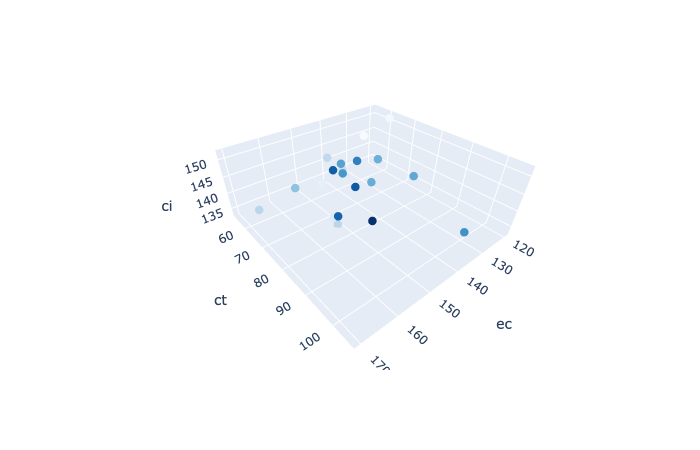
\includegraphics[width=1.2\linewidth]{images/ga-dem8.png}
			\caption{Gamma - T8}\label{fig:nsga-ii-ga-dem8}
		\end{minipage}
	\end{figure}

	\begin{figure}[H]
		\begin{minipage}{0.5\textwidth}
			\centering
			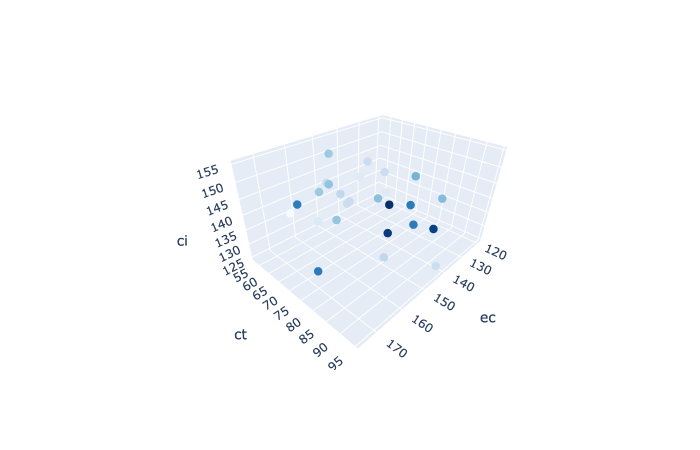
\includegraphics[width=1.2\linewidth]{images/ga-dem9.png}
			\caption{Gamma - T9}\label{fig:nsga-ii-ga-dem9}
		\end{minipage}\hfill
		\begin{minipage}{0.5\textwidth}
			\centering
			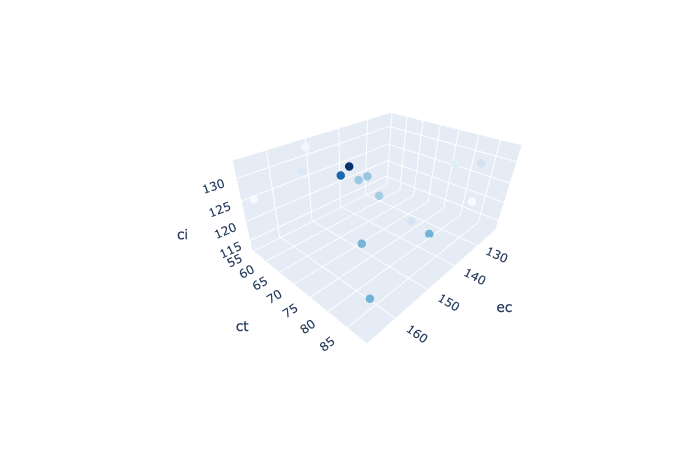
\includegraphics[width=1.2\linewidth]{images/ga-dem10.png}
			\caption{Gamma - T10}\label{fig:nsga-ii-ga-dem10}
		\end{minipage}
	\end{figure}
	
	\item Phân phối Chuẩn
	\begin{figure}[H]
		\begin{minipage}{0.5\textwidth}
			\centering
			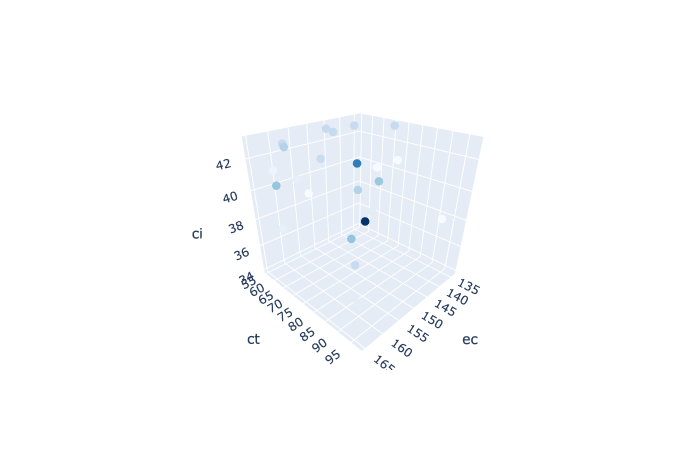
\includegraphics[width=1.2\linewidth]{images/no-dem1.png}
			\caption{No - T1}\label{fig:nsga-ii-no-dem1}
		\end{minipage}\hfill
		\begin{minipage}{0.5\textwidth}
			\centering
			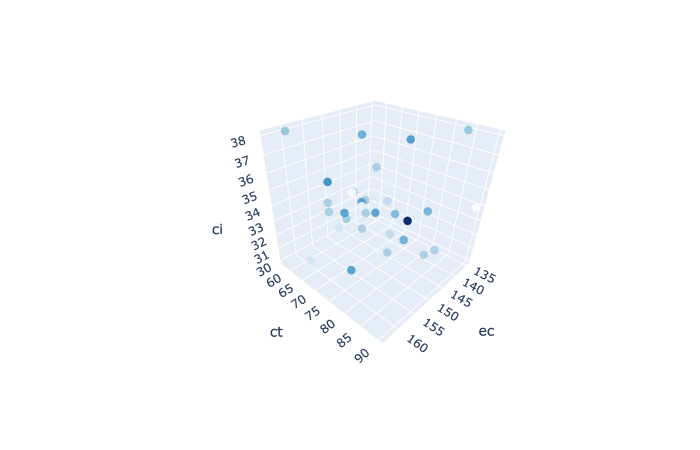
\includegraphics[width=1.2\linewidth]{images/no-dem2.png}
			\caption{No - T2}\label{fig:nsga-ii-no-dem2}
		\end{minipage}
	\end{figure}
	
	\begin{figure}[H]
		\begin{minipage}{0.5\textwidth}
			\centering
			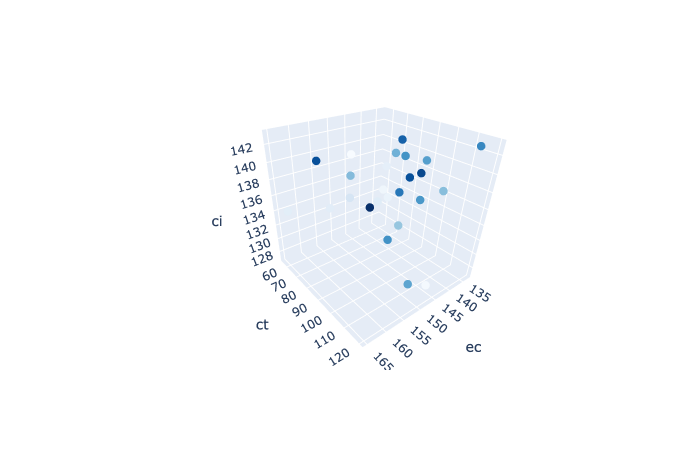
\includegraphics[width=1.2\linewidth]{images/no-dem3.png}
			\caption{No - T3}\label{fig:nsga-ii-no-dem3}
		\end{minipage}\hfill
		\begin{minipage}{0.5\textwidth}
			\centering
			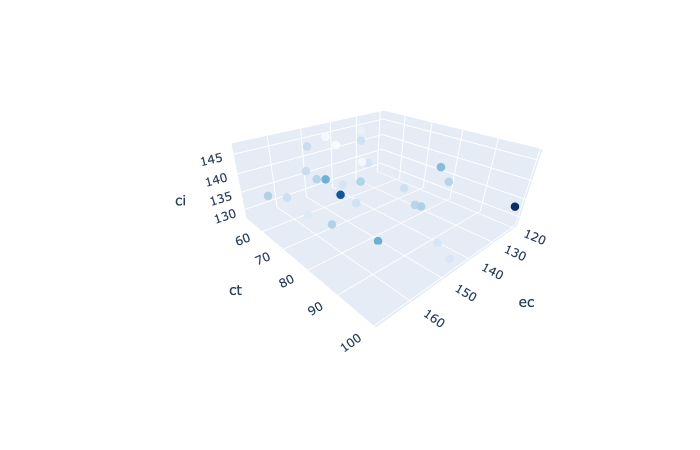
\includegraphics[width=1.2\linewidth]{images/no-dem4.png}
			\caption{No - T4}\label{fig:nsga-ii-no-dem4}
		\end{minipage}
	\end{figure}
	
	\begin{figure}[H]
		\begin{minipage}{0.5\textwidth}
			\centering
			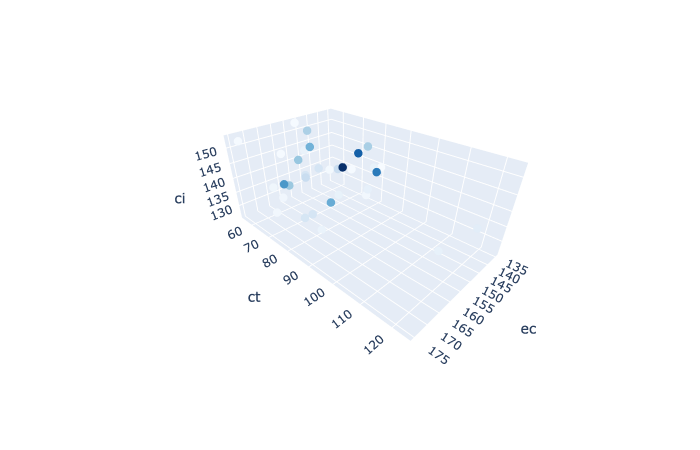
\includegraphics[width=1.2\linewidth]{images/no-dem5.png}
			\caption{No - T5}\label{fig:nsga-ii-no-dem5}
		\end{minipage}\hfill
		\begin{minipage}{0.5\textwidth}
			\centering
			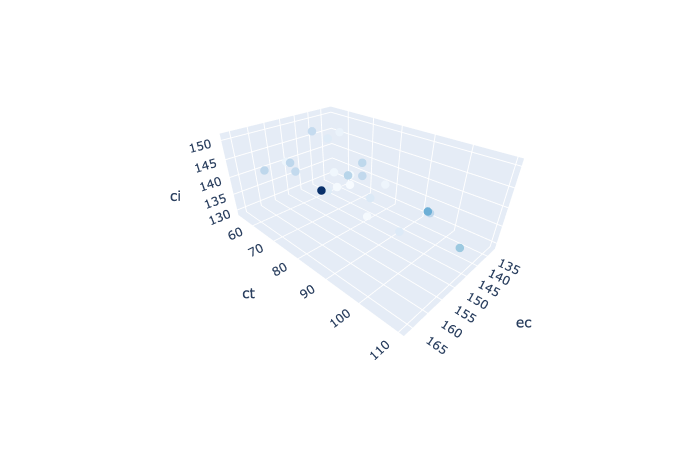
\includegraphics[width=1.2\linewidth]{images/no-dem6.png}
			\caption{No - T6}\label{fig:nsga-ii-no-dem6}
		\end{minipage}
	\end{figure}
	
	\begin{figure}[H]
		\begin{minipage}{0.5\textwidth}
			\centering
			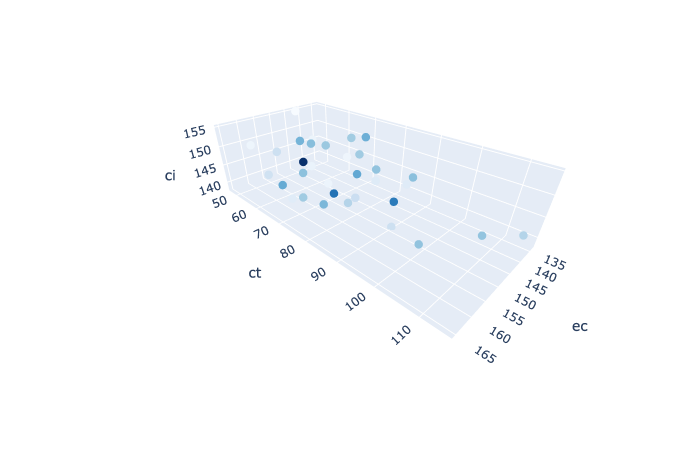
\includegraphics[width=1.2\linewidth]{images/no-dem7.png}
			\caption{No - T7}\label{fig:nsga-ii-no-dem7}
		\end{minipage}\hfill
		\begin{minipage}{0.5\textwidth}
			\centering
			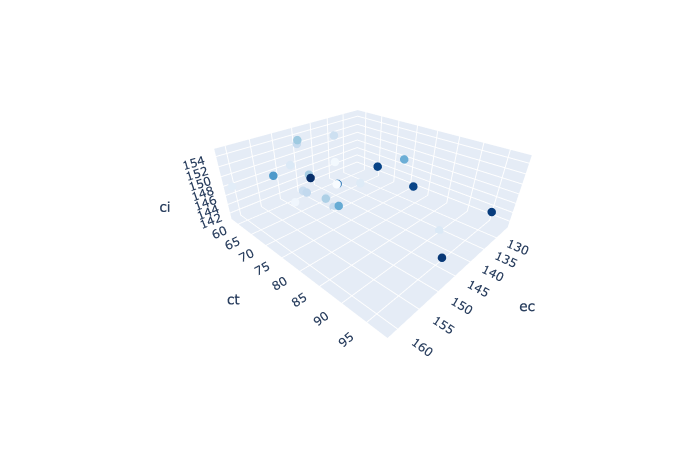
\includegraphics[width=1.2\linewidth]{images/no-dem8.png}
			\caption{No - T8}\label{fig:nsga-ii-no-dem8}
		\end{minipage}
	\end{figure}
	
	\begin{figure}[H]
		\begin{minipage}{0.5\textwidth}
			\centering
			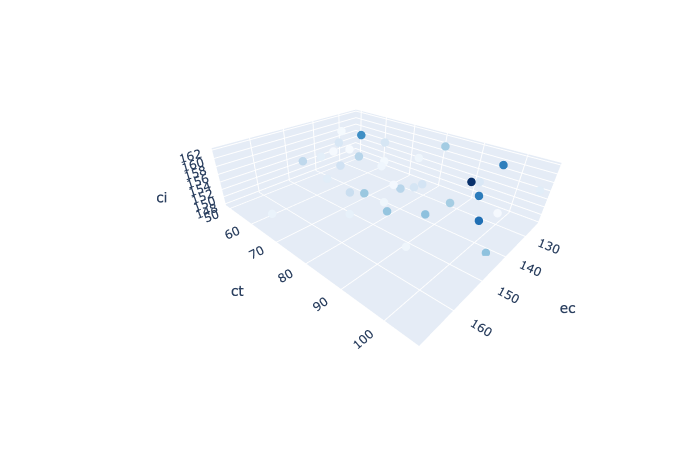
\includegraphics[width=1.2\linewidth]{images/no-dem9.png}
			\caption{No - T9}\label{fig:nsga-ii-no-dem9}
		\end{minipage}\hfill
		\begin{minipage}{0.5\textwidth}
			\centering
			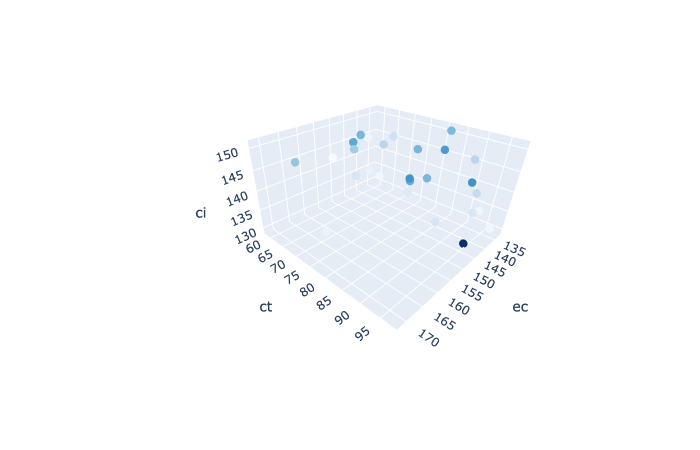
\includegraphics[width=1.2\linewidth]{images/no-dem10.png}
			\caption{No - T10}\label{fig:nsga-ii-no-dem10}
		\end{minipage}
	\end{figure}

	\item Phân phối Đều
	\begin{figure}[H]
		\begin{minipage}{0.5\textwidth}
			\centering
			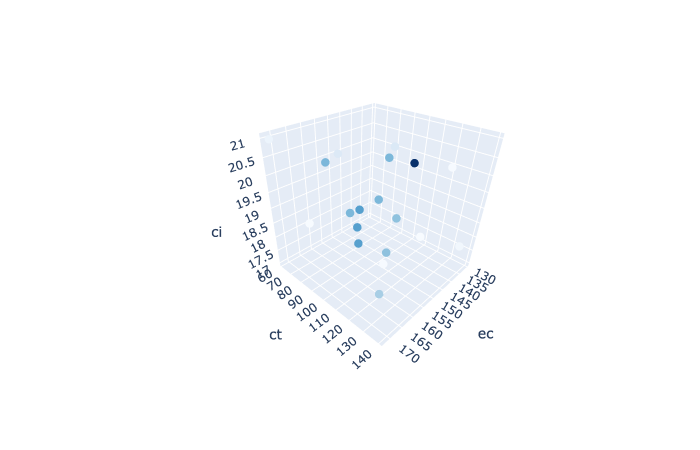
\includegraphics[width=1.2\linewidth]{images/uu-dem1.png}
			\caption{Uniform - T1}\label{fig:nsga-ii-uu-dem1}
		\end{minipage}\hfill
		\begin{minipage}{0.5\textwidth}
			\centering
			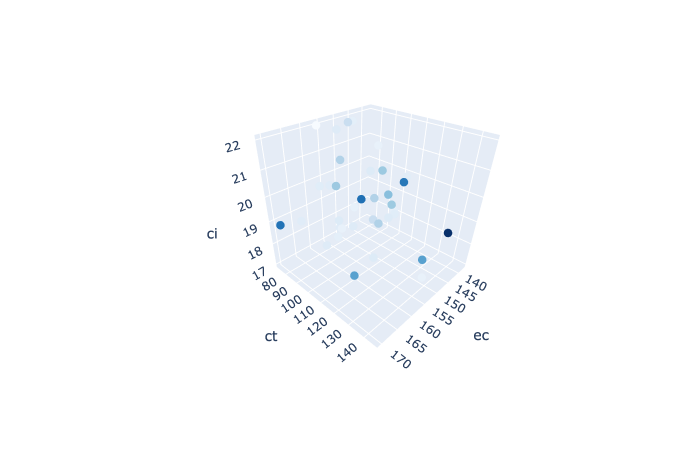
\includegraphics[width=1.2\linewidth]{images/uu-dem2.png}
			\caption{Uniform - T2}\label{fig:nsga-ii-uu-dem2}
		\end{minipage}
	\end{figure}
	
	\begin{figure}[H]
		\begin{minipage}{0.5\textwidth}
			\centering
			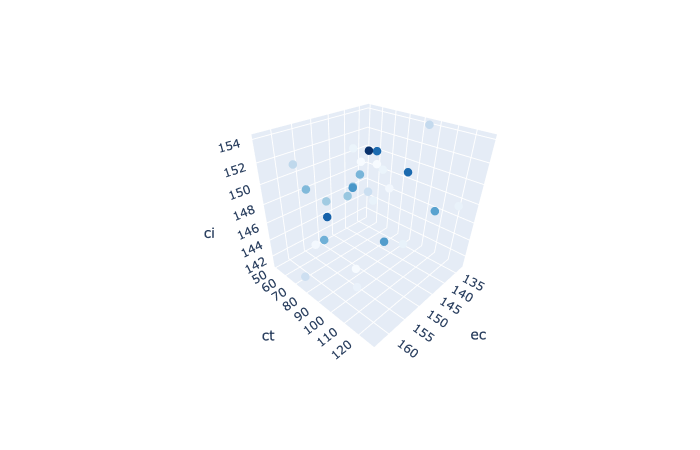
\includegraphics[width=1.2\linewidth]{images/uu-dem3.png}
			\caption{Uniform - T3}\label{fig:nsga-ii-uu-dem3}
		\end{minipage}\hfill
		\begin{minipage}{0.5\textwidth}
			\centering
			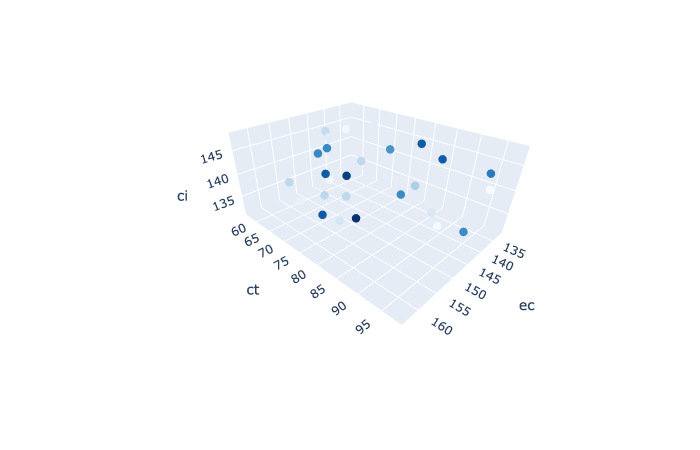
\includegraphics[width=1.2\linewidth]{images/uu-dem4.png}
			\caption{Uniform - T4}\label{fig:nsga-ii-uu-dem4}
		\end{minipage}
	\end{figure}
	
	\begin{figure}[H]
		\begin{minipage}{0.5\textwidth}
			\centering
			\includegraphics[width=1.2\linewidth]{images/uu-dem5.png}
			\caption{Uniform - T5}\label{fig:nsga-ii-uu-dem5}
		\end{minipage}\hfill
		\begin{minipage}{0.5\textwidth}
			\centering
			\includegraphics[width=1.2\linewidth]{images/uu-dem6.png}
			\caption{Uniform - T6}\label{fig:nsga-ii-uu-dem6}
		\end{minipage}
	\end{figure}
	
	\begin{figure}[H]
		\begin{minipage}{0.5\textwidth}
			\centering
			\includegraphics[width=1.2\linewidth]{images/uu-dem7.png}
			\caption{Uniform - T7}\label{fig:nsga-ii-uu-dem7}
		\end{minipage}\hfill
		\begin{minipage}{0.5\textwidth}
			\centering
			\includegraphics[width=1.2\linewidth]{images/uu-dem8.png}
			\caption{Uniform - T8}\label{fig:nsga-ii-uu-dem8}
		\end{minipage}
	\end{figure}
	
	\begin{figure}[H]
		\begin{minipage}{0.5\textwidth}
			\centering
			\includegraphics[width=1.2\linewidth]{images/uu-dem9.png}
			\caption{Uniform - T9}\label{fig:nsga-ii-uu-dem9}
		\end{minipage}\hfill
		\begin{minipage}{0.5\textwidth}
			\centering
			\includegraphics[width=1.2\linewidth]{images/uu-dem10.png}
			\caption{Uniform - T10}\label{fig:nsga-ii-uu-dem10}
		\end{minipage}
	\end{figure}
\end{itemize}

\chapter*{Kết luận}
Đồ án tập trung nghiên cứu về giải thuật tiến hoá trên mạng cảm biến không dây, cụ thể là giải thuật di truyền và giải thuật di truyền sắp xếp không trội. Kiến thức tổng quan về mạng cảm biến không dây, bao gồm kiến trúc các loại mạng cảm biến, cấu trúc một nút cảm biến được đề cập ở chương 1, các mục tiêu được quan tâm và nghiên cứu của đồ án được đề cập ở chương 2. Chương 3 và chương 4 là phần giải thích và trình bày kết quả khi thực nghiệm với hai giải thuật, giải thuật di truyền và giải thuật di truyền sắp xếp không trội.


Đồ án có thể được mở rộng theo ba hướng. Hướng thứ nhất là áp dụng các giải thuật tiến hoá đa mục tiêu khác trên bộ dữ liệu hiện có để so sánh với kết quả hiện tại, lựa chọn giải thuật mang lại kết quả tốt nhất. Hướng thứ hai là thay đổi quy trình thực hiện của hai giải thuật đã áp dụng, có thể thay đổi ở bước mã hoá, lai ghép hoặc đột biến. Hướng còn lại là kết hợp từ cả hai hướng trên.


Dẫu còn nhiều thiếu sót cần cải thiện, đồ án đã đóng góp một phần nhỏ trong lĩnh vực nghiên cứu sử dụng giải thuật tiến hoá nhằm tối ưu các mục tiêu trên mạng cảm biến không dây.

\bibliographystyle{plain}
\bibliography{ref}
\end{document}
s